\documentclass[12pt]{article}

\usepackage[utf8]{inputenc}
\usepackage[T1]{fontenc}
\usepackage[spanish]{babel}
\usepackage{cmbright}
\usepackage{lmodern}
\usepackage{geometry}
\usepackage{pgfplots}
\usepackage{tikz}
\usetikzlibrary{positioning,calc,math,arrows.meta,decorations.markings,intersections}
\usepackage{hyperref}
\usepackage[bf,sf,pagestyles]{titlesec}
\usepackage{titling}
\usepackage[runin]{abstract}
\usepackage[font={footnotesize, sf}, labelfont=bf]{caption} 
\usepackage{siunitx}
\usepackage{graphicx}
\usepackage{booktabs}
\usepackage{multirow}
\usepackage{amsmath,amssymb}
\usepackage[spanish,sort]{cleveref}
\usepackage{enumitem}

\geometry{
	a4paper,
	right = 2.5cm,
	left = 2.5cm,
	bottom = 3cm,
	top = 3cm
}

\newcommand{\sfbright}{\fontfamily{cmbr}\selectfont}
\renewcommand{\familydefault}{\rmdefault}
\renewcommand{\sfdefault}{cmbr}
\renewcommand{\arraystretch}{1.4}

\hypersetup{
	colorlinks,
	linkcolor = {red!50!blue},
	citecolor = {red!50!blue},
	linktoc = page
}

\numberwithin{table}{section}
\numberwithin{figure}{section}
\numberwithin{equation}{section}

\graphicspath{{./figs/}}

% Unitats
\sisetup{
	inter-unit-product = \ensuremath{ \, },
	allow-number-unit-breaks = true,
	math-celsius = {}^{\circ}\kern-\scriptspace C,
	detect-family = true,
	mode = text,
	list-final-separator = { y },
	list-pair-separator = { y },
	list-units = single,
	separate-uncertainty = true
}

\newcommand{\Z}{\mathbb{Z}}
\newcommand{\N}{\mathbb{N}}
\newcommand{\R}{\mathbb{R}}
\newcommand{\Ry}{\mathit{Ry}}
\newcommand{\conv}[2]{\filldraw[fill = white!50!-red, fill opacity = 0.5, draw = -red!] (#1,0) ellipse [x radius = 0.1, y radius = #2];}
\newcommand{\data}[3]{\SI{#1 \pm #2}{#3}}
\newcommand{\unc}[2]{\ensuremath{{}\pm \SI{#1}{#2}}}
\DeclareMathOperator{\sen}{sin}
\newcommand{\abs}[1]{\left\lvert #1 \right\rvert}
\newcommand{\inn}[2]{\left\langle #1 , #2 \right\rangle}
\newcommand{\parbreak}{
	\begin{center}
		--- $\ast$ ---
	\end{center} 
}
\makeatletter
\newcommand*{\defeq}{\mathrel{\rlap{%
		\raisebox{0.3ex}{$\m@th\cdot$}}%
	\raisebox{-0.3ex}{$\m@th\cdot$}}%
	=
}
\makeatother

\newpagestyle{pagina}{
	\headrule
	\sethead*{\sffamily \bfseries Práctica 2}{}{\theauthor}
	\footrule
	\setfoot*{}{}{\sffamily \thepage}
}
\renewpagestyle{plain}{
	\footrule
	\setfoot*{}{}{\sffamily \thepage}
}
\pagestyle{pagina}

\title{\sffamily {\bfseries Práctica 2:} Reflexión y refracción en dioptrios planos. Efecto Pffund}
\author{\sffamily B2 2: Arnau Mas, Alejandro Plaza}
\date{\sffamily 28 de febrero de 2019}

\begin{document}
\maketitle
\renewcommand{\abstractname}{\sffamily \bfseries Resumen:}
\begin{abstract}
	En esta práctica se utiliza la refracción de la luz en dioptrios planos para calcular satisfactoriamente el índice de refracción de una lámina de vidrio.
	
	También se estudia el efecto Pffund sobre diversos materiales, con el cual se evidencian la reflexión y la refracción de la luz en superficies de separación entre dos medios. Gracias a este efecto se consigue calcular el índice de refracción de una lámina de vidrio y del agua.
\end{abstract}
\hrule

\section{Objetivos}
En esta práctica se estudiarán en general la reflexión y la refracción de la luz. Se comprobarán las leyes que gobiernan estos fenómenos.

En la primera parte se verá involucrada la formación de imágenes y se verá la influencia de lo paraxiales que sean los rayos de luz en estas imágenes

Se utilizará la refracción para medir el índice de refracción de una lámina vítrea.

En la segunda parte se utilizará el concepto de reflexión total y ángulo límite para observar el efecto Pffund en una lámina de líquido.

\section{Índice de refracción de una lámina}
En esta parte de la práctica se medirá el índice de refracción de una placa de vidrio.

Cuando se tienen dos medios de distintos índices de refracción separados por un dioptrio plano, si se coloca un objeto en el primer medio y se observa desde el otro; el efecto es el mismo que si se tuviese una imagen del objeto ---de otro tamaño y en otra posición--- y los rayos surgiesen de esta imagen y se propagasen sin desviarse.

\begin{figure}[!ht]
	\small \centering \sffamily
	\begin{center}
		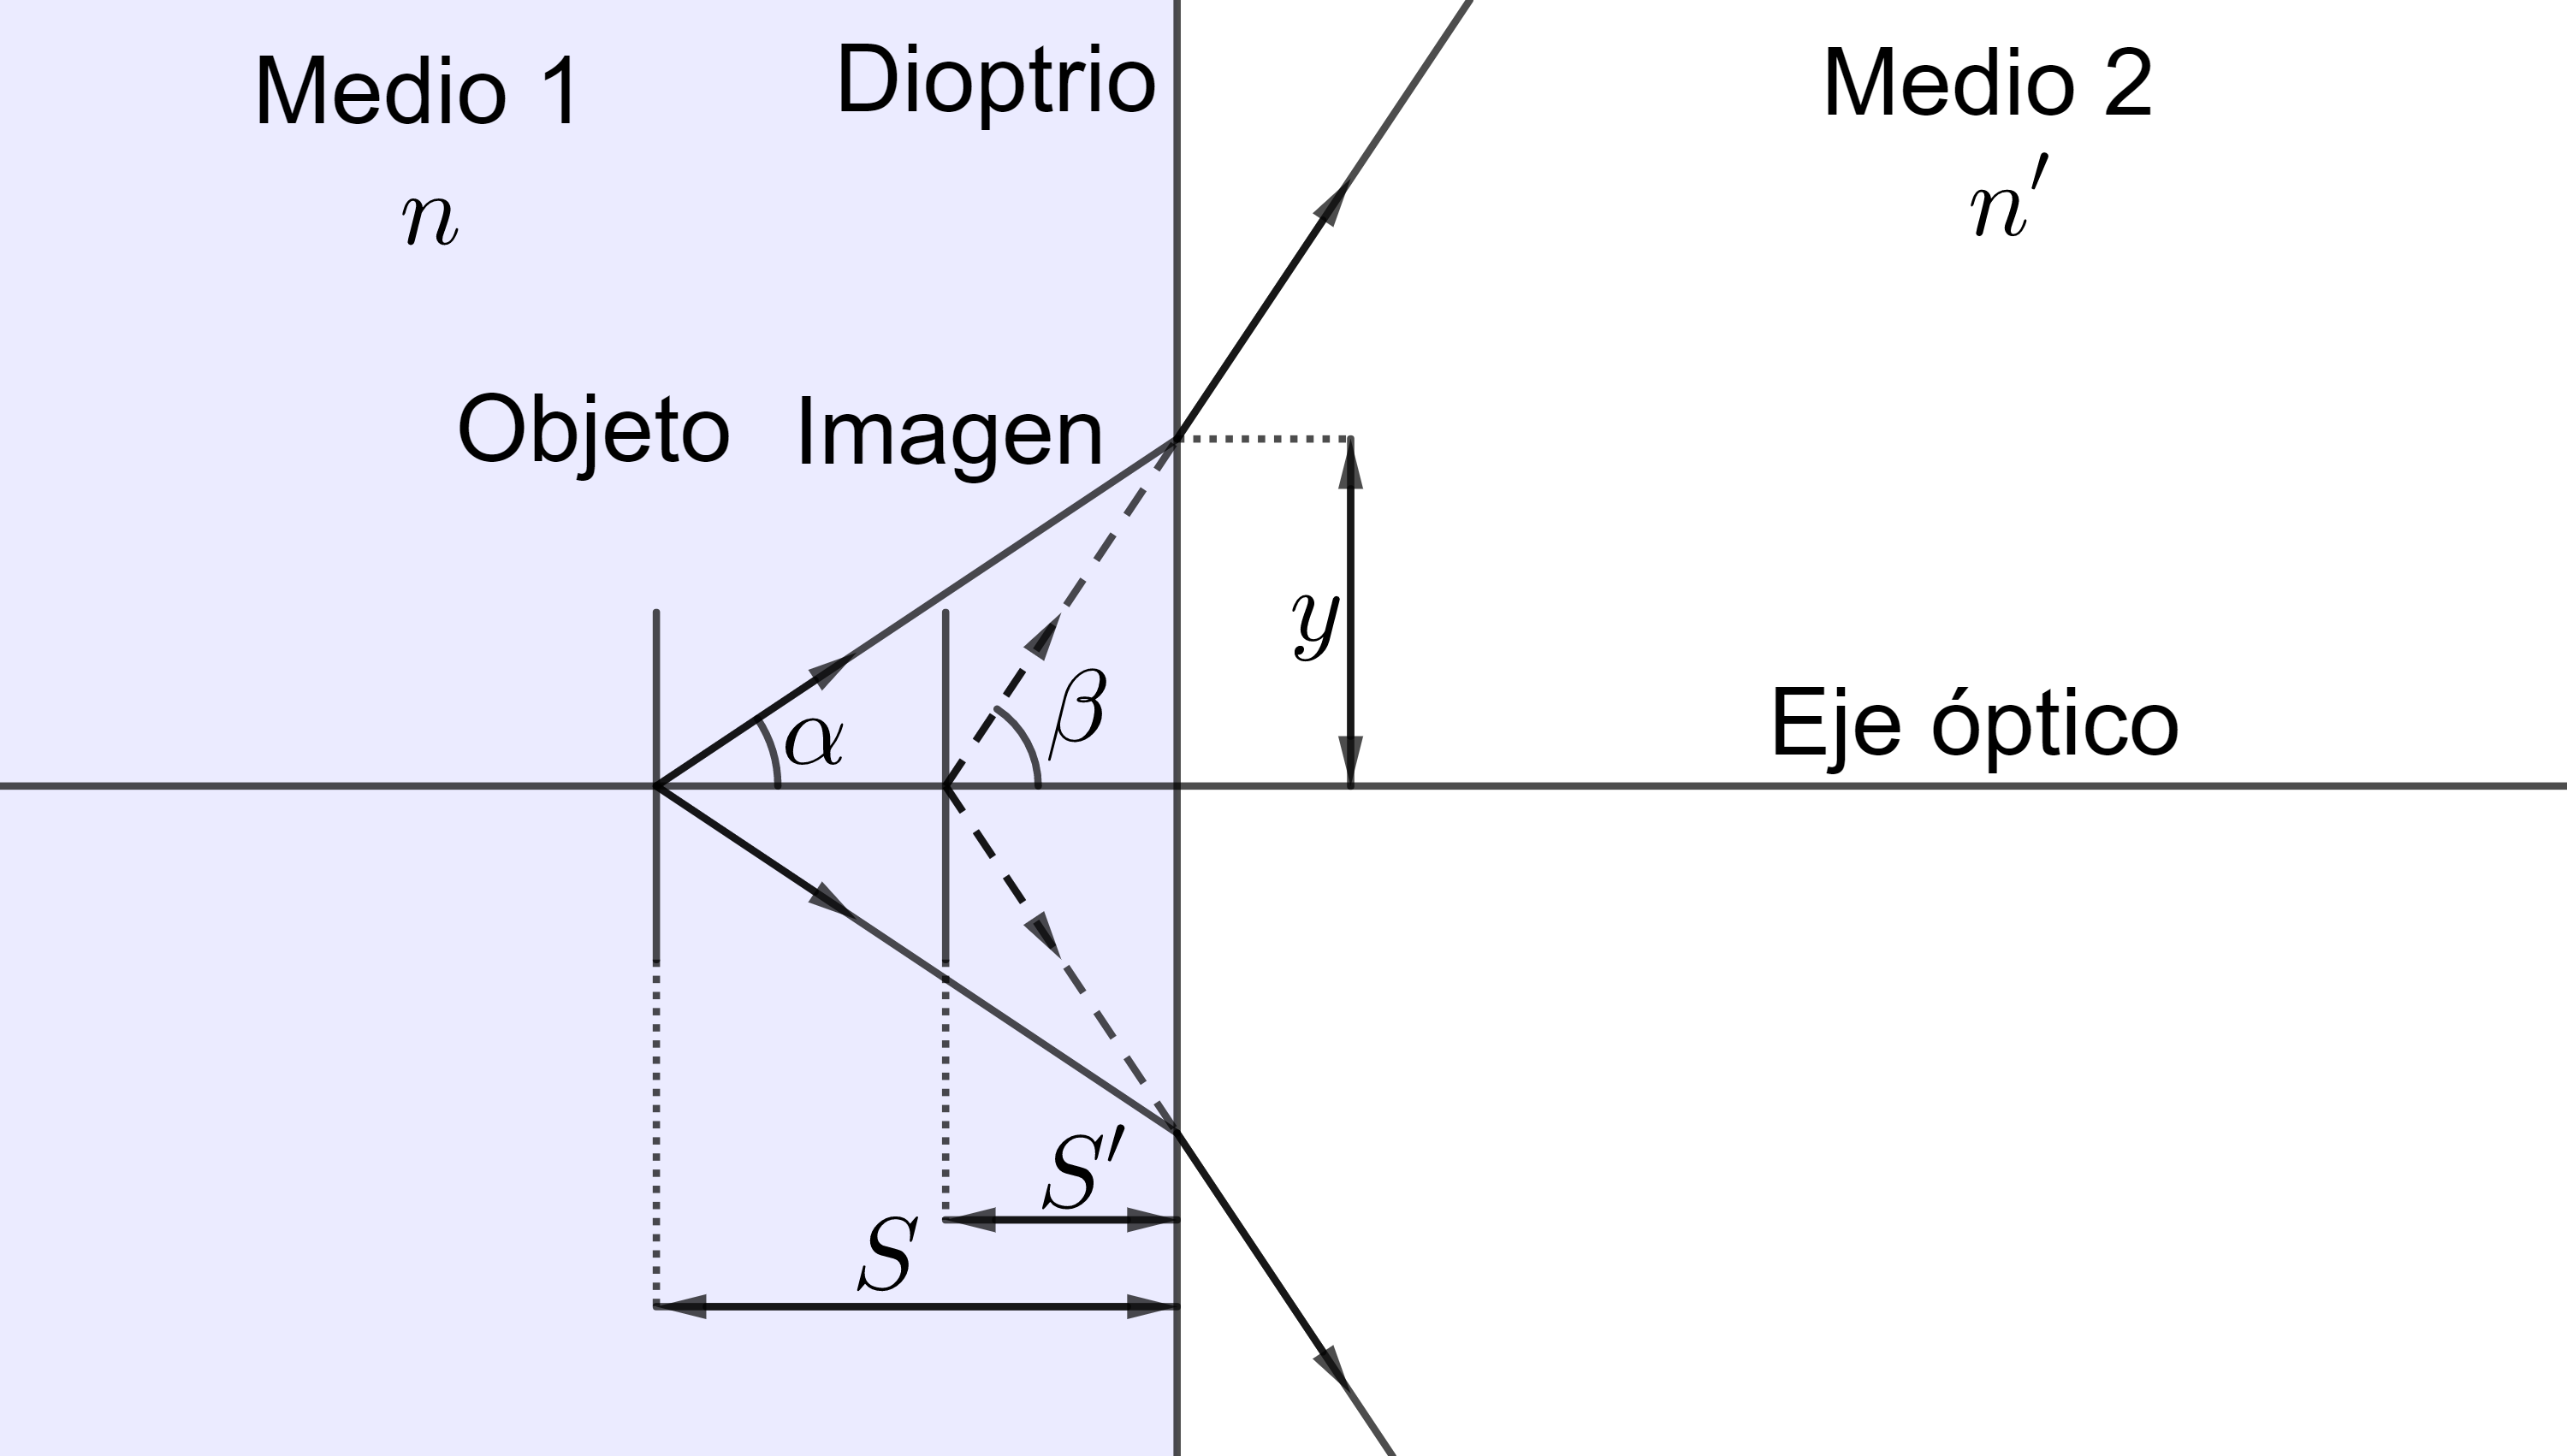
\includegraphics[width=10cm]{P2Refraccion.png}
		\caption{Esquema de la imagen formada por refracción en un dioptrio plano.}
		\label{P2refraccion}
	\end{center}
\end{figure}

En la figura \ref{P2refraccion} se ve un esquema de lo que ocurre, donde $s$ es la distancia del objeto al dioptrio y $s'$ es la distancia de la imagen al dioptrio. La ley de Snell nos dice que $\frac{\sen\alpha}{\sen\beta}=\frac{n'}{n}$. Por trigonometría tenemos $\tan\alpha=\frac{y}{s}$ y $\tan\beta=\frac{y}{s'}$, que se resume en $\frac{\tan\alpha}{\tan\beta}=\frac{s'}{s}$. En el caso paraxial ---es decir, para rayos que forman un ángulo pequeño con el eje óptico--- los ángulos $\alpha$ y $\beta$ son muy pequeños se puede hacer la aproximación $\sen\alpha\approx\tan\alpha$ y $\sen\beta\approx\tan\alpha$, con lo que queda $\frac{n'}{n}=\frac{\sen\alpha}{\sen\beta}\approx\frac{\tan\alpha}{\tan\beta}=\frac{s'}{s}$.
\begin{equation}\label{P2distimagen}
	s'=\frac{n'}{n}s
\end{equation} 

Sin embargo esta expresión es aproximada, pues según el ángulo con que sale un rayo del objeto, su imagen está en un sitio u otro como se ve en la figura \ref{P2astigmatismo}. Pero los rayos paraxiales forman la imagen todos ellos casi en el mismo sitio.

\begin{figure}[!ht]
	\small \centering \sffamily
	\begin{center}
		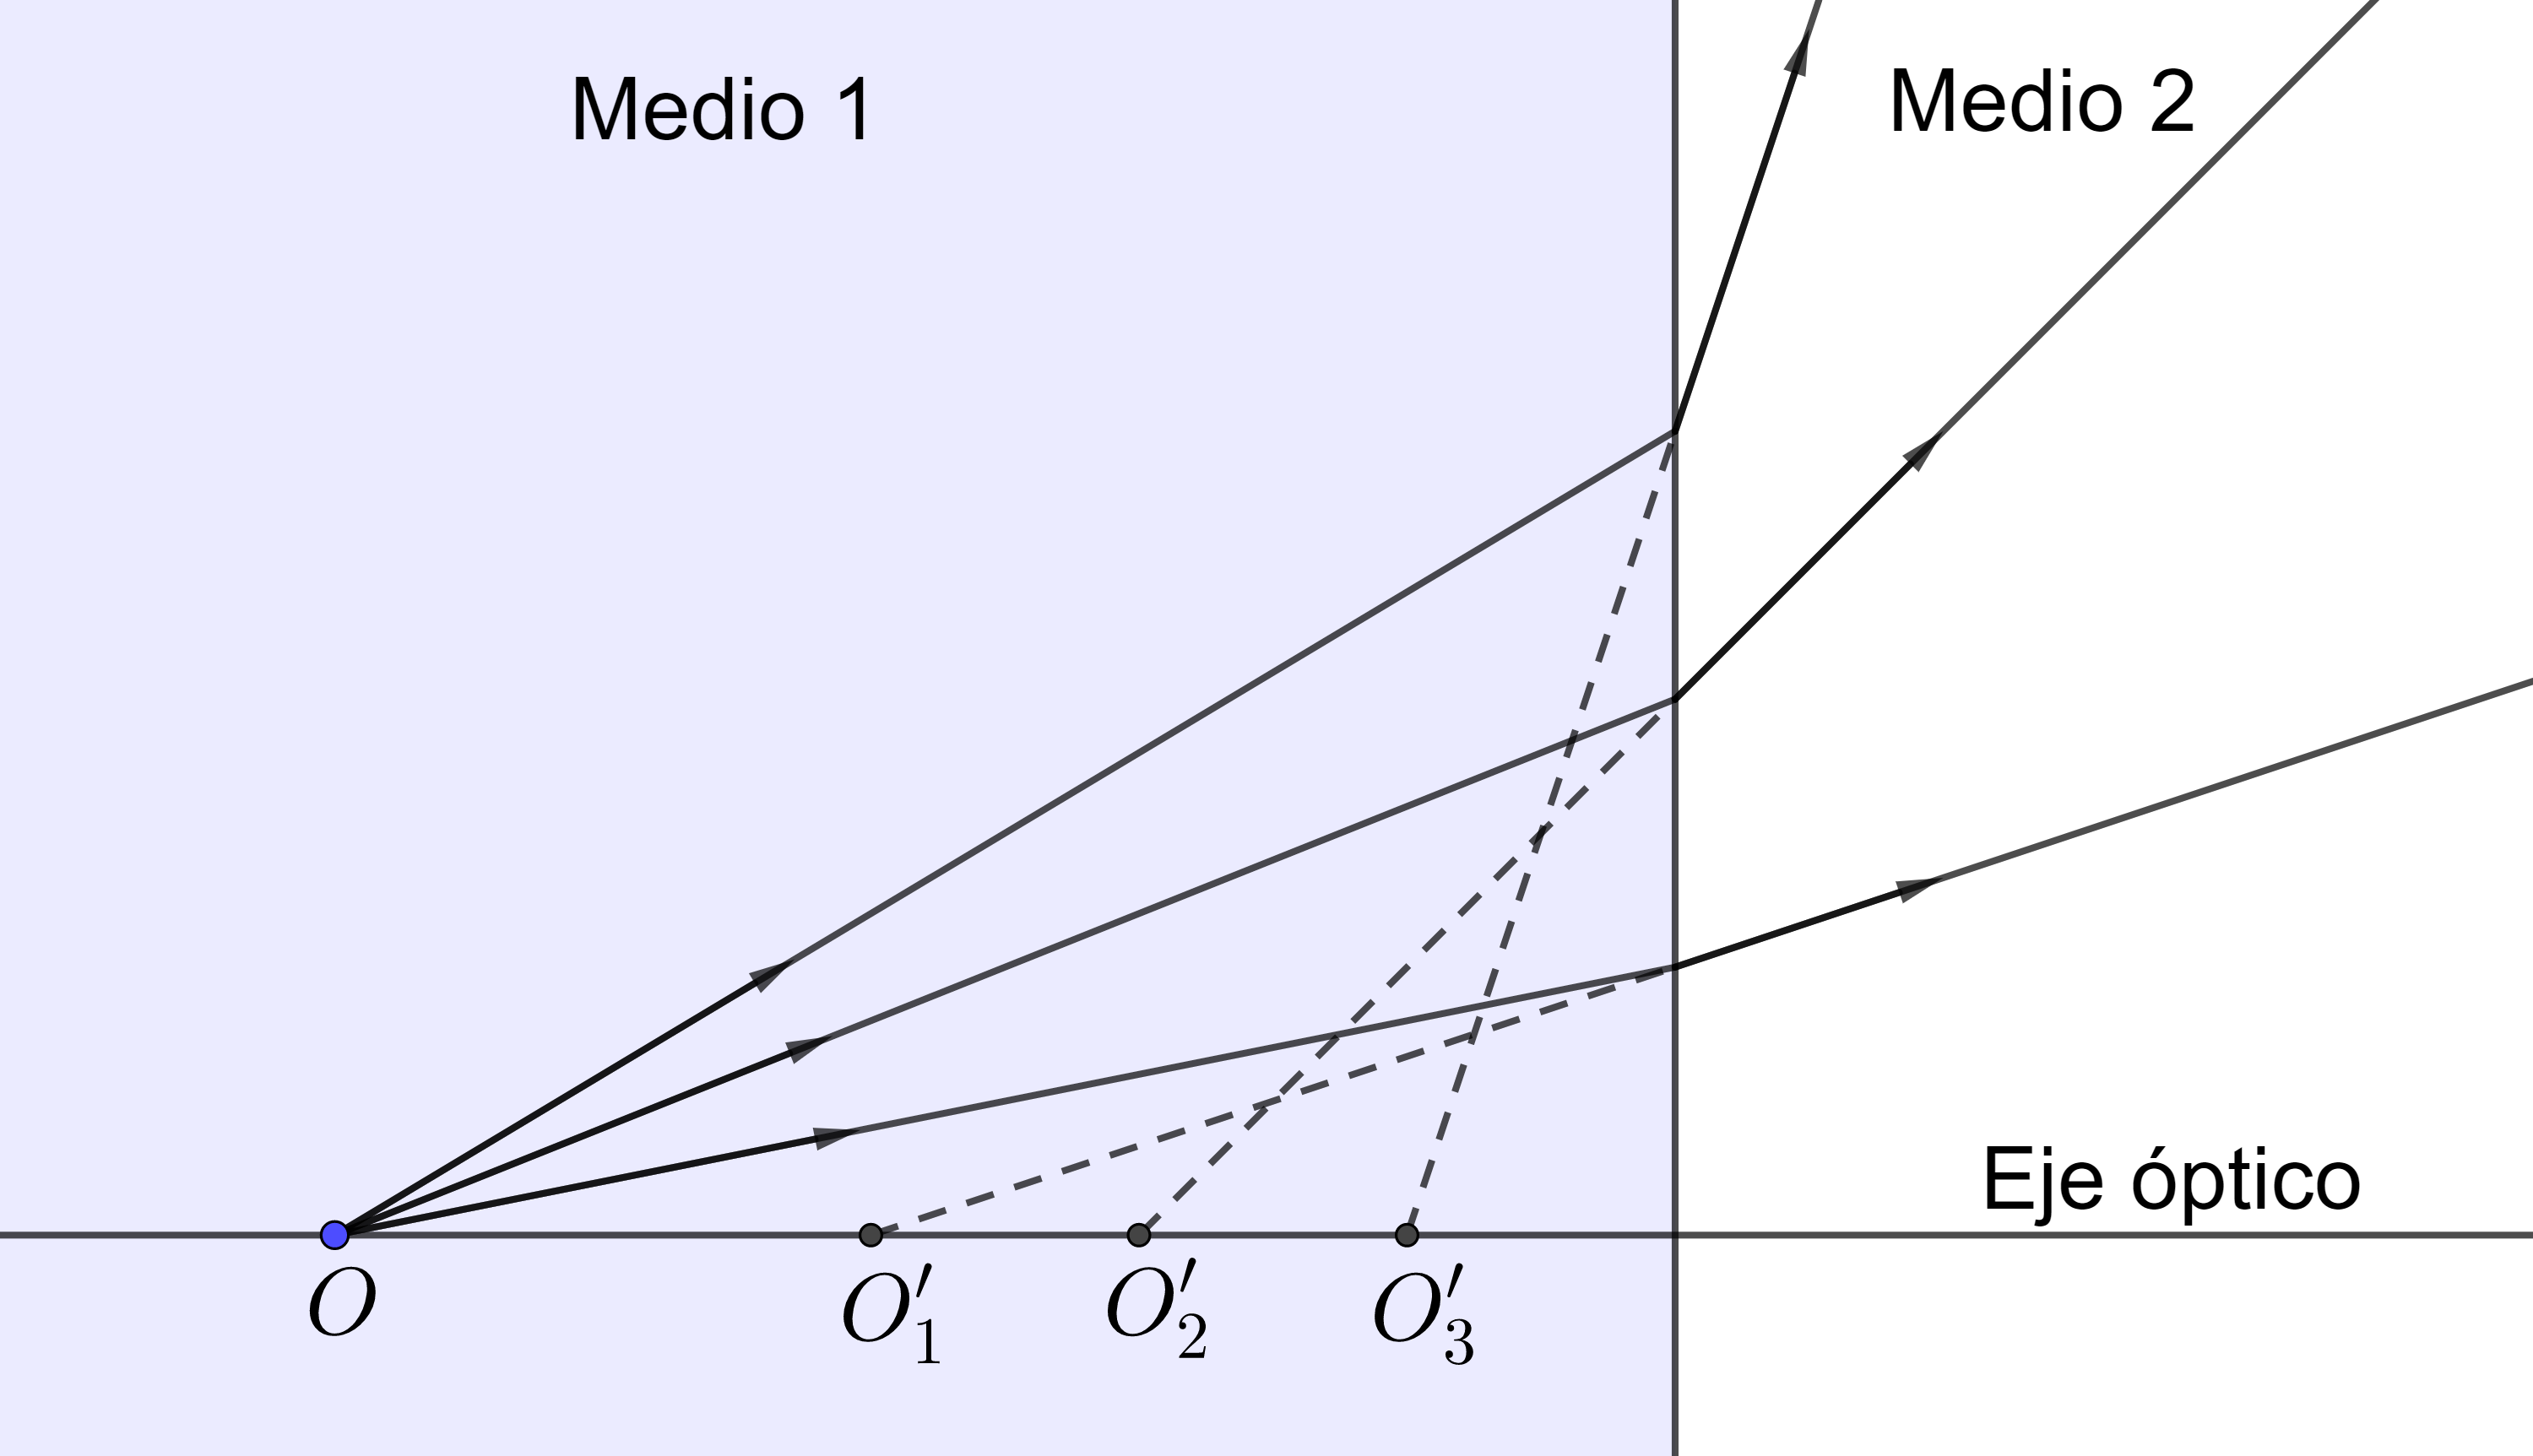
\includegraphics[width=10cm]{P2Astigmatismo.png}
		\caption{Esquema de las distintas imágenes formadas por refracción en un dioptrio plano según el ángulo de inclinación de los rayos.}
		\label{P2astigmatismo}
	\end{center}
\end{figure}

Cuando se forma una imagen clara y nítida se dice que el dioptrio es estigmático.

Se quiere utilizar la ecuación (\ref{P2distimagen}) para calcular el índice de refracción de una lámina de vidrio. Para ello se pintan unas rayas en ambas caras de la lámina. Una de las rayas actuará de objeto y el grosor de la lámina será la distancia que separe el objeto del dioptrio $s$. Este dioptrio separa dos medios: vidrio y aire; por lo tanto, $n'$ será el índice de refracción del aire, el cual consideraremos, 0 y $n$ será el índice del vidrio.

El grosor de la lámina se mide con un comparador: se coloca la lámina en la platina y se miden las posiciones de la platina y de la parte superior de la lámina. Su diferencia será el grosor buscado. Se realizan varias medidas con el fin de disminuir la incertidumbre. La incertidumbre de cada medida directa es la precisión del comparador: $ \SI{0.010}{mm}$. La de la diferencia es la anterior multiplicada por $\sqrt{2}$ como indica la fórmula (\ref{P2incdif}). El valor que se tomará es el de la media aritmética, con incertidumbre calculada según (\ref{P2incmedia}).

\begin{table}[!ht]
	\small \centering \sffamily
	\caption{Tabla con las medidas de las posiciones de la platina y la lámina ---con incertidumbre $ \SI{0.010}{mm}$--- junto a su diferencia ---con incertidumbre \SI{0.014}{mm}---, que es el grosor de la lámina. Todas las medidas están en milímetros.}
	\label{P2tablaverdadero}
	\begin{center}
		\begin{tabular}{@{}rSSSSS@{}}
			\toprule
			&{Medida 1}&{Medida 2}&{Medida 3}&{Medida 4}&{Medida 5}\\
			\midrule
			Posición 1 (\unc{0.010}{mm})&11.870&11.880&11.860&11.900&11.890\\
			Posición 2 (\unc{0.010}{mm})&26.480&26.510&26.490&26.540&26.520\\
			\midrule
			Diferencia (\unc{0.014}{mm})&14.610&14.630&14.630&14.640&14.630\\
			\bottomrule
		\end{tabular}
	\end{center}
\end{table}

En la tabla \ref{P2tablaverdadero} se encuentran estas medidas, de las que se deduce que el grosor medio de la placa es \( s = \data{14.628}{0.014}{mm} \)

Ahora se mide la distancia de la imagen al dioptrio. Para ello se utiliza un microscopio y se calcula restando la posición de la platina a la que se enfoca el objeto visto a través del vidrio y la posición de la misma a la que se enfoca un dibujo pintado en la cara superior.

El microscopio tiene dos diafragmas: el diafragma de campo y el diafragma de apertura. El primero regula el área iluminada: el círculo iluminado será tanto mayor cuanto más abierto esté el diafragma y viceversa. Se sitúa en la parte inferior del microscopio. El segundo controla la inclinación de los rayos: al cerrarse el diafragma se dejan pasar únicamente los rayos más paraxiales.

Con el microscopio de que se dispone para esta práctica se comprueba que al abrir y cerrar el diafragma de la base del microscopio se amplía y se reduce el círculo iluminado en la muestra, lo que quiere decir que es el de campo.

Con el otro diafragma, el área iluminada se ve más iluminada o menos según se abre y se cierra. La muestra se ve igual de enfocada con este diafragma abierto o cerrado porque el desenfoque que produce que los rayos no sean del todo paraxiales no es muy grande. Sin embargo el que cambie cuánto está iluminado indica que se dejan pasar más rayos o menos, pues al limitar el paso a solo los rayos paraxiales; los que no lo son dejan de iluminar la muestra. Por lo tanto este diafragma es el de apertura.

Cuando los rayos que llegan al microscopio son paraxiales, se es capaz de conseguir un mejor enfoque, pues el sistema es estigmático y la imagen que se forma es muy nítida. Sin embargo existe una amplia región del espacio donde al colocar la muestra se ve bastante bien enfocada. Por su parte, cuando los rayos son oblicuos, el máximo enfoque posible no es tan bueno como el que se conseguiría con los rayos paraxiales y además la región del espacio en la que se puede enfocar medianamente bien está mucho más concentrada alrededor del plano focal.

No obstante, que los rayos no sean paraxiales será útil en esta práctica porque lo que interesa no es conseguir un enfoque perfecto, sino saber con precisión en qué punto se enfoca bien.

\begin{table}[!ht]
	\footnotesize \centering \sffamily
	\caption{Tabla con las medidas de las posiciones aparentes de las caras superior e inferior de la lámina de vidrio ---con incertidumbre \SI{0.010}{mm}--- junto a su diferencia ---con incertidumbre \SI{0.014}{mm}---, que es el grosor aparente de la lámina. Todas las medidas están en milímetros. Las primeras medidas están hechas con el diafragma de apertura cerrado y después con el diafragma abierto.}
	\label{P2tablaaparente}
	\begin{tabular}{ccSSSSS}
		\toprule
		&&{Medida 1}&{Medida 2}&{Medida 3}&{Medida 4}&{Medida 5}\\
		\midrule
		\multirow{3}{*}{Cerrado}&Posición 1 (\unc{0.010}{mm}) &16.260&16.030&16.400&15.970&15.120\\
														&Posición 2 (\unc{0.010}{mm})&25.980&25.620&25.700&25.660&25.650\\
		\cmidrule{2-7}
		&Diferencia (\unc{0.014}{mm})&9.720&9.590&9.300&9.690&10.530\\
		\midrule
		\multirow{3}{*}{Abierto}&Posición 1 (\unc{0.010}{mm})&16.260&16.050&16.100&15.990&16.150\\
														&Posición 2 (\unc{0.010}{mm})&25.700&25.580&25.680&25.730&25.820\\
		\cmidrule{2-7}
		&Diferencia (\unc{0.014}{mm})&9.440&9.530&9.580&9.740&9.670 \\
		\bottomrule
	\end{tabular}
\end{table}

En la tabla \ref{P2tablaaparente} se encuentran las medidas del grosor aparente de la placa con el diafragma de apertura abierto y cerrado. La media del grosor con el diafragma cerrado es \data{9.766}{0.044}{mm} y con el diafragma abierto es \data{9.592}{0.014}{mm}. Se puede apreciar que la incertidumbre con el diafragma abierto es aproximadamente tres veces menor que con el diafragma cerrado. Esta diferencia es más acusada si se observan las desviaciones típicas de las medias ---debidas únicamente a la dispersión de las medidas, sin tener en cuenta la precisión del aparato de medida---. La desviación típica con el diafragma cerrado es \SI{0.042}{mm} y abierto es \SI{0.0028}{mm}, unas 15 veces menor.

Esto confirma lo que se había dicho antes: cuando se abre el diafragma la región donde el objeto se ve enfocado se reduce y por lo tanto las medidas se concentran más alrededor de la media.

El índice de refracción de un material depende de la longitud de onda, produciéndose una dispersión cromática. Para comprobar esta dependencia en la lámina de vidrio, se verá cómo varían las medidas en función de la longitud de onda de la luz utilizada. Para ello se colocará un filtro que transmite la luz roja y un filtro que transmite la luz azul, dos colores con longitudes de onda lo más dispares posible dentro del rango visible.

Se ha visto que con el diafragma de apertura abierto se obtienen unos resultados más precisos, de modo que para esta parte de la práctica se deja el diafragma abierto.

\begin{table}[!ht]
	\small \centering \sffamily
	\caption{Tabla con las medidas de las posiciones aparentes de las caras superior e inferior de la lámina de vidrio ---con incertidumbre \SI{0.010}{mm}--- junto a su diferencia ---con incertidumbre \SI{0.014}{mm}---, que es el grosor aparente de la lámina. Todas las medidas están en milímetros. Las primeras medidas están hechas con un filtro rojo y después con un filtro azul.}
	\label{P2tablacolores}
	\begin{tabular}{ccSSS}
		&&{Medida 1}&{Medida 2}&{Medida 3}\\
		\midrule
		\multirow{3}{*}{Rojo}&Posición 1 (\unc{0.010}{mm}) &15.680&15.510&15.580\\
												 &Posición 2 (\unc{0.010}{mm})&25.200&25.080&25.260\\
		\cmidrule{2-5}
		&Diferencia (\unc{0.014}{mm})&9.520&9.570&9.680\\
		\midrule
		\multirow{3}{*}{Azul}&Posición 1 (\unc{0.010}{mm})&15.650&15.510&15.570\\
												 &Posición 2 (\unc{0.010}{mm})&25.090&24.950&25.180\\
		\cmidrule{2-5}
		&Diferencia (\unc{0.014}{mm})&9.440&9.440&9.610 \\
		\bottomrule
	\end{tabular}
\end{table}

La media del grosor con el filtro rojo es \data{9.590}{0.014}{mm} y con el azul es \data{9.497}{0.015}{mm}. Vemos que no son compatibles, lo que quiere decir que se pueden considerar distintas. La dispersión cromática en esta lámina de vidrio no es despreciable.

Finalmente se calcula el índice de refracción de la lámina de vidrio usada en esta práctica gracias a la fórmula (\ref{P2distimagen}). Su incertidumbre es calculada mediante la fórmula de propagación de incertidumbres. Sin poner ningún filtro con el diafragma abierto el índice calculado es \num{1.5250\pm0.0027}. El índice de refracción para la longitud de onda del rojo vale \num{1.5253\pm0.0027} y para el azul \num{1.5403\pm0.0028}. Efectivamente el índice de refracción es distinto para cada longitud de onda. Cuando no se pone ningún filtro el índice de refracción es muy parecido al del rojo. Esto ocurre porque el objeto que se ha usado era de color rojo, de modo que la luz proveniente del objeto era mayoritariamente roja.

Con el diafragma cerrado se tiene un índice de refracción igual a \num{1.4978\pm0.0069}, que dista mucho de los tres valores anteriores por las razones ya explicadas.

\section{Efecto Pffund}
Cuando se hace incidir un rayo de luz sobre una superficie y se refleja, puede salir reflejado de dos formas principalmente: especular y difusa. La primera se produce cuando la superficie es pulida y sale formando el mismo ángulo con la normal. La segunda ocurre cuando la superficie es rugosa.

En realidad la reflexión es siempre especular, pero cuando la superficie es rugosa, en cada punto la normal puede tener cualquier inclinación y por lo tanto al final el rayo puede ser reflejado en cualquier dirección.

Para esta práctica se utiliza un láser. Primero se observarán una serie de cosas para entender mejor la propagación rectilínea de la luz y la reflexión especular y difusa.

El láser se dispone para que su luz salga horizontal. Se utiliza un espejo a \SI{45}{\degree} para hacer que el haz caiga perpendicular sobre la mesa. Entre el espejo y la mesa se pone una lente que focaliza la luz. Al encender el láser, el rayo de luz no se ve, pues solo se ven los puntos desde los que sale un rayo que llega al ojo. Se ve principalmente el punto de la mesa al que llega el haz de luz y se refleja difusamente. Sin embargo también se ven puntos muy débiles en el espejo y en la lente que no deberían verse, pero hay una fracción mínima de la luz que se refleja de forma difusa y acaba llegando al ojo.

Ahora se apunta con el láser al espejo por la cara de aluminio. Esta cara es pulida y opaca, por lo que toda la luz que incide es reflejada de forma especular. Al apuntar, sin embargo, se ve un punto rojo muy débil. Como antes, una pequeña parte del rayo es reflejado difusamente y llega al ojo.

Cuando se apunta con el láser al papel satinado una parte se refleja y otra parte se refracta a partes quizá no iguales, pero sí similares. El papel es rugoso, así pues la reflexión y la transmisión son difusas, es decir, el rayo sale en todas las direcciones. Gracias a esto en cualquier posición el rayo llega al ojo y se ve un punto rojo en el punto donde incide el láser. Cuando se mira el papel por el lado en el que está el láser, la luz llega al ojo por reflexión. Cuando se mira por el lado donde no está el láser, el rayo llega al ojo refractándose en el papel.

Con el plástico blanco, como es opaco, la luz no lo atraviesa: no se refracta. Solo se refleja y lo hace de forma especular. Cuando se mira detrás del plástico no se ve nada y si se mira la cara enfrentada al aparato láser, se ve un punto rojo fruto de la reflexión difusa.

Se dispone de un espejo óptico que en un lado tiene aluminio pulido y opaco que refleja la luz de modo especular. El otro lado es de un vidrio que transmite la luz. Cuando el haz incide sobre la cara vítrea, una parte es reflejada y otra es transmitida al interior. Al llegar a la cara de aluminio se refleja y después llega otra vez a la superficie vidrio-aire y parte es transferida al exterior y otra parte se queda reflejada en el interior. Cada vez que se refleja la luz en la cara de vidrio, pierde intensidad porque parte de la luz se está transmitiendo. Se puede ver un esquema de lo que ocurre en la figura \ref{P2espejo}.

\begin{figure}[!ht]
	\small \centering \sffamily
	\begin{center}
		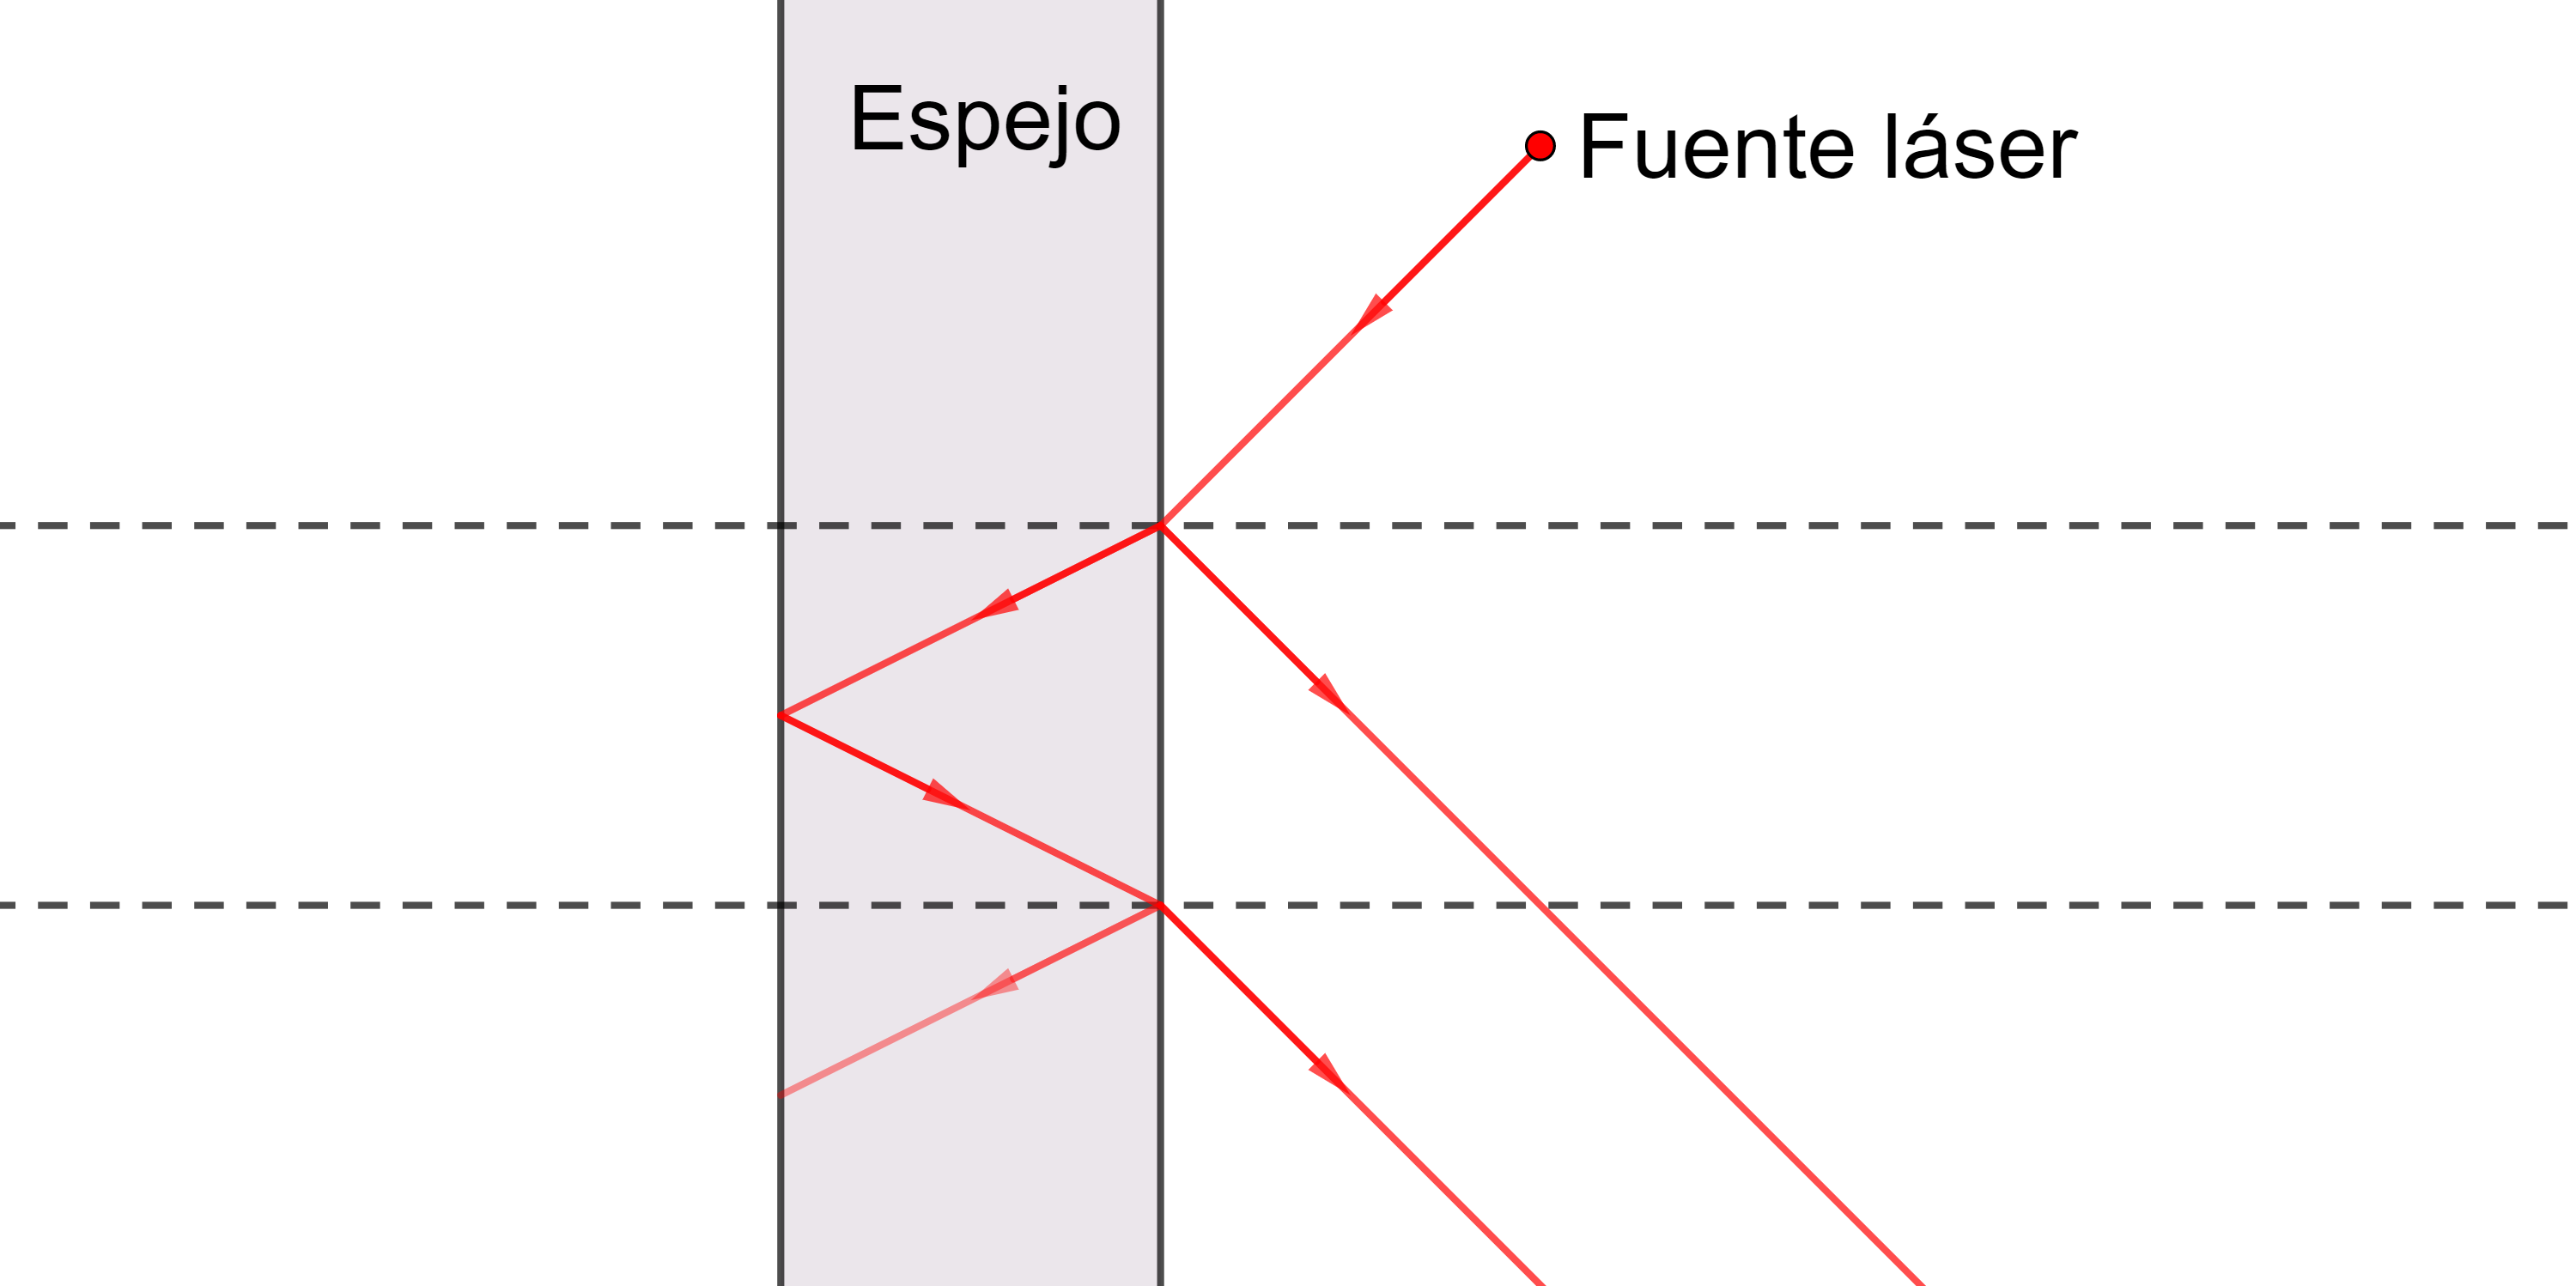
\includegraphics[width=8cm]{P2Espejo.png}
		\caption{Esquema de un haz de luz láser que entra a un espejo con una cara izquierda opaca y con el resto de vidrio.}
		\label{P2espejo}
	\end{center}
\end{figure}

Cuando se proyecta la luz del láser sobre el espejo se observan un punto intenso y cinco puntos a su alrededor más débiles. El punto central es el rayo procedente del laser que se refracta en la cara de vidrio, se refleja en la cara de aluminio y luego se vuelve a refractar saliendo al exterior. Los otros son resultado del rayo anterior que, en su última refracción, en lugar de salir al aire, se refleja otra vez, va hasta la cara opaca del espejo, se refleja y al final se refracta en la cara del vidrio y sale. Estos últimos puntos son más débiles por la pérdida de intensidad comentada en el parágrafo anterior.

Al inclinar el espejo los puntos se ven más brillantes porque cuando los rayos llegan a la superficie vidrio-aire desde la parte del vidrio lo hacen con un ángulo de incidencia mayor, más próximo al ángulo límite. Por lo tanto se refleja más luz que antes y llega más luz a los puntos que rodean el punto central. Por esto se ven más brillantes.

Por la ley de Snell si un rayo de luz llega a una superficie de separación entre dos medios con índices de refracción $n$ y $n'$ y forma un ángulo $\varepsilon$ con la recta normal a la superficie, el rayo saldrá desviado formando un ángulo $\varepsilon'$ con la normal.
\begin{equation}\label{P2Snell}
	\frac{\sen\varepsilon'}{\sen\varepsilon}=\frac{n}{n'}
\end{equation}
Otra forma de escribir (\ref{P2Snell}) es $\sen\varepsilon'=\frac{n}{n'}\sen\varepsilon$. Si $n>n'$, existirá un ángulo de incidencia $\varepsilon$ tal que el rayo refracto forme un ángulo $\varepsilon'= {\frac{\pi}{2}}\si{rad}$. Este ángulo se conoce como ángulo límite $\varepsilon_l$. En este caso $\sen\varepsilon'=1$.
\begin{equation}\label{P2eqangulolimite}
	\sen\varepsilon_l=\frac{n'}{n}
\end{equation}
Este ángulo existe porque por hipótesis $\frac{n'}{n}<1$. Si el ángulo de incidencia es mayor que el ángulo límite $\epsilon>\epsilon_l$, entonces $\sen\varepsilon>\sen\varepsilon_l$ y $\sen\varepsilon'=\frac{n}{n'}\sen\varepsilon>\frac{n}{n'}\sen\varepsilon_l>\frac{n}{n'}\frac{n'}{n}=1$. Sin embargo no existe ningún ángulo real cuyo seno sea mayor que 1. Por lo tanto si el ángulo de incidencia es mayor que el ángulo límite, no existirá un rayo transmitido: todo el rayo será reflejado. Este fenómeno se conoce como reflexión total y se puede ver un esquema en la figura \ref{P2figangulolimite}.

\begin{figure}[!ht]
	\small \centering \sffamily
	\begin{center}
		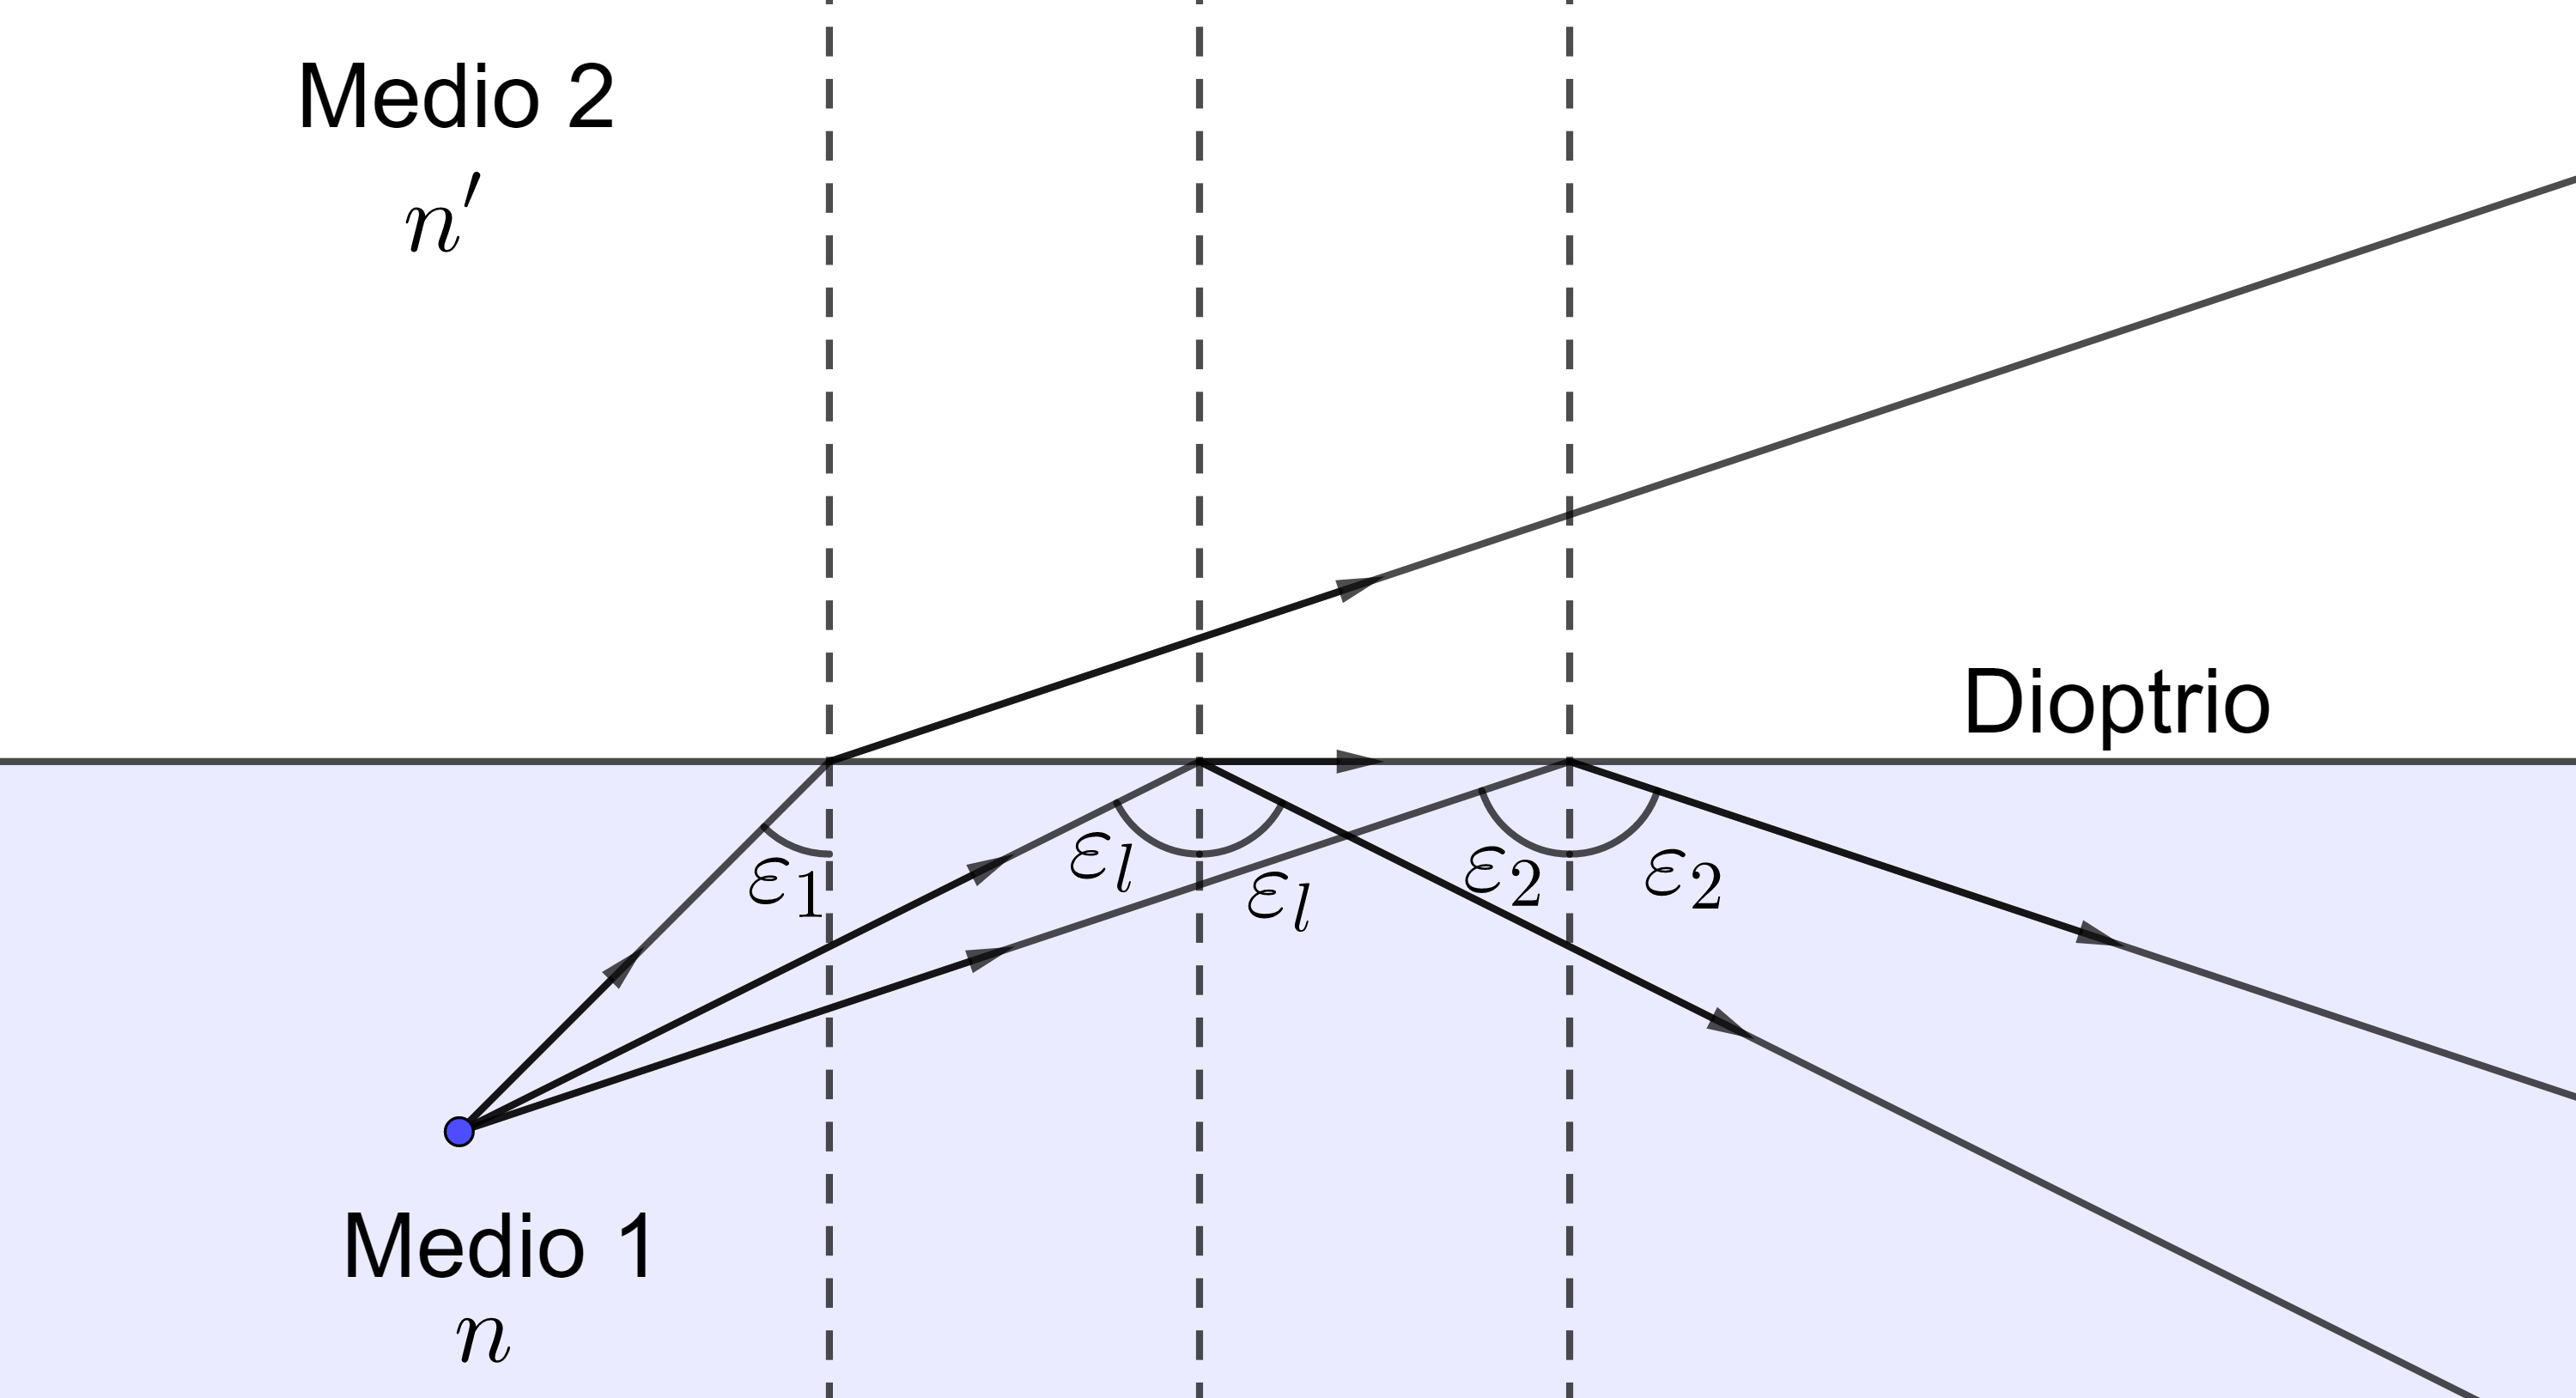
\includegraphics[width=10cm]{P2Angulolimite.png}
		\caption{Esquema de la reflexión y refracción de rayos con distinto ángulo de incidencia. Cuando este supera el ángulo límite, el rayo es reflejado íntegramente.}
		\label{P2figangulolimite}
	\end{center}
\end{figure}

Siempre que un rayo de luz llega a un dioptrio, una fracción es refractada y la fracción complementaria es reflejada. Cuando $n>n'$, conforme aumenta el ángulo de incidencia, la fracción refractada se va haciendo cada vez más pequeña en favor de la reflejada. Hasta que se llega al ángulo límite, a partir del cual todo el rayo es reflejado.

El concepto de reflexión total es en el que se basa el efecto Pffund.

Se vierte agua sobre la mesa y se forma una fina lámina plana de agua. La luz del láser cae verticalmente sobre el agua y llega a la mesa en el punto $A$ de la figura \ref{P2PffAgua}. Ahí se refleja de forma difusa en todas las direcciones, entre ellas la que llega al ojo. Ese punto se ve iluminado. De ahí los rayos que salen poco inclinados llegan a la superficie y se refractan casi enteramente y muy poca parte del rayo se refleja. El rayo que sale del punto $A$ con un ángulo de inclinación igual al ángulo límite, ---el cual existe porque el índice del agua es mayor que el del aire---, llega al punto $B$ y se refleja íntegro de forma especular llegando al punto $C$, donde se refleja de forma difusa y este punto se ve iluminado. Los rayos que tienen una inclinación mayor que el ángulo límite también se reflejan íntegros y llegan a la mesa más allá del punto $C$.

\begin{figure}[!ht]
	\small \centering \sffamily
	\begin{center}
		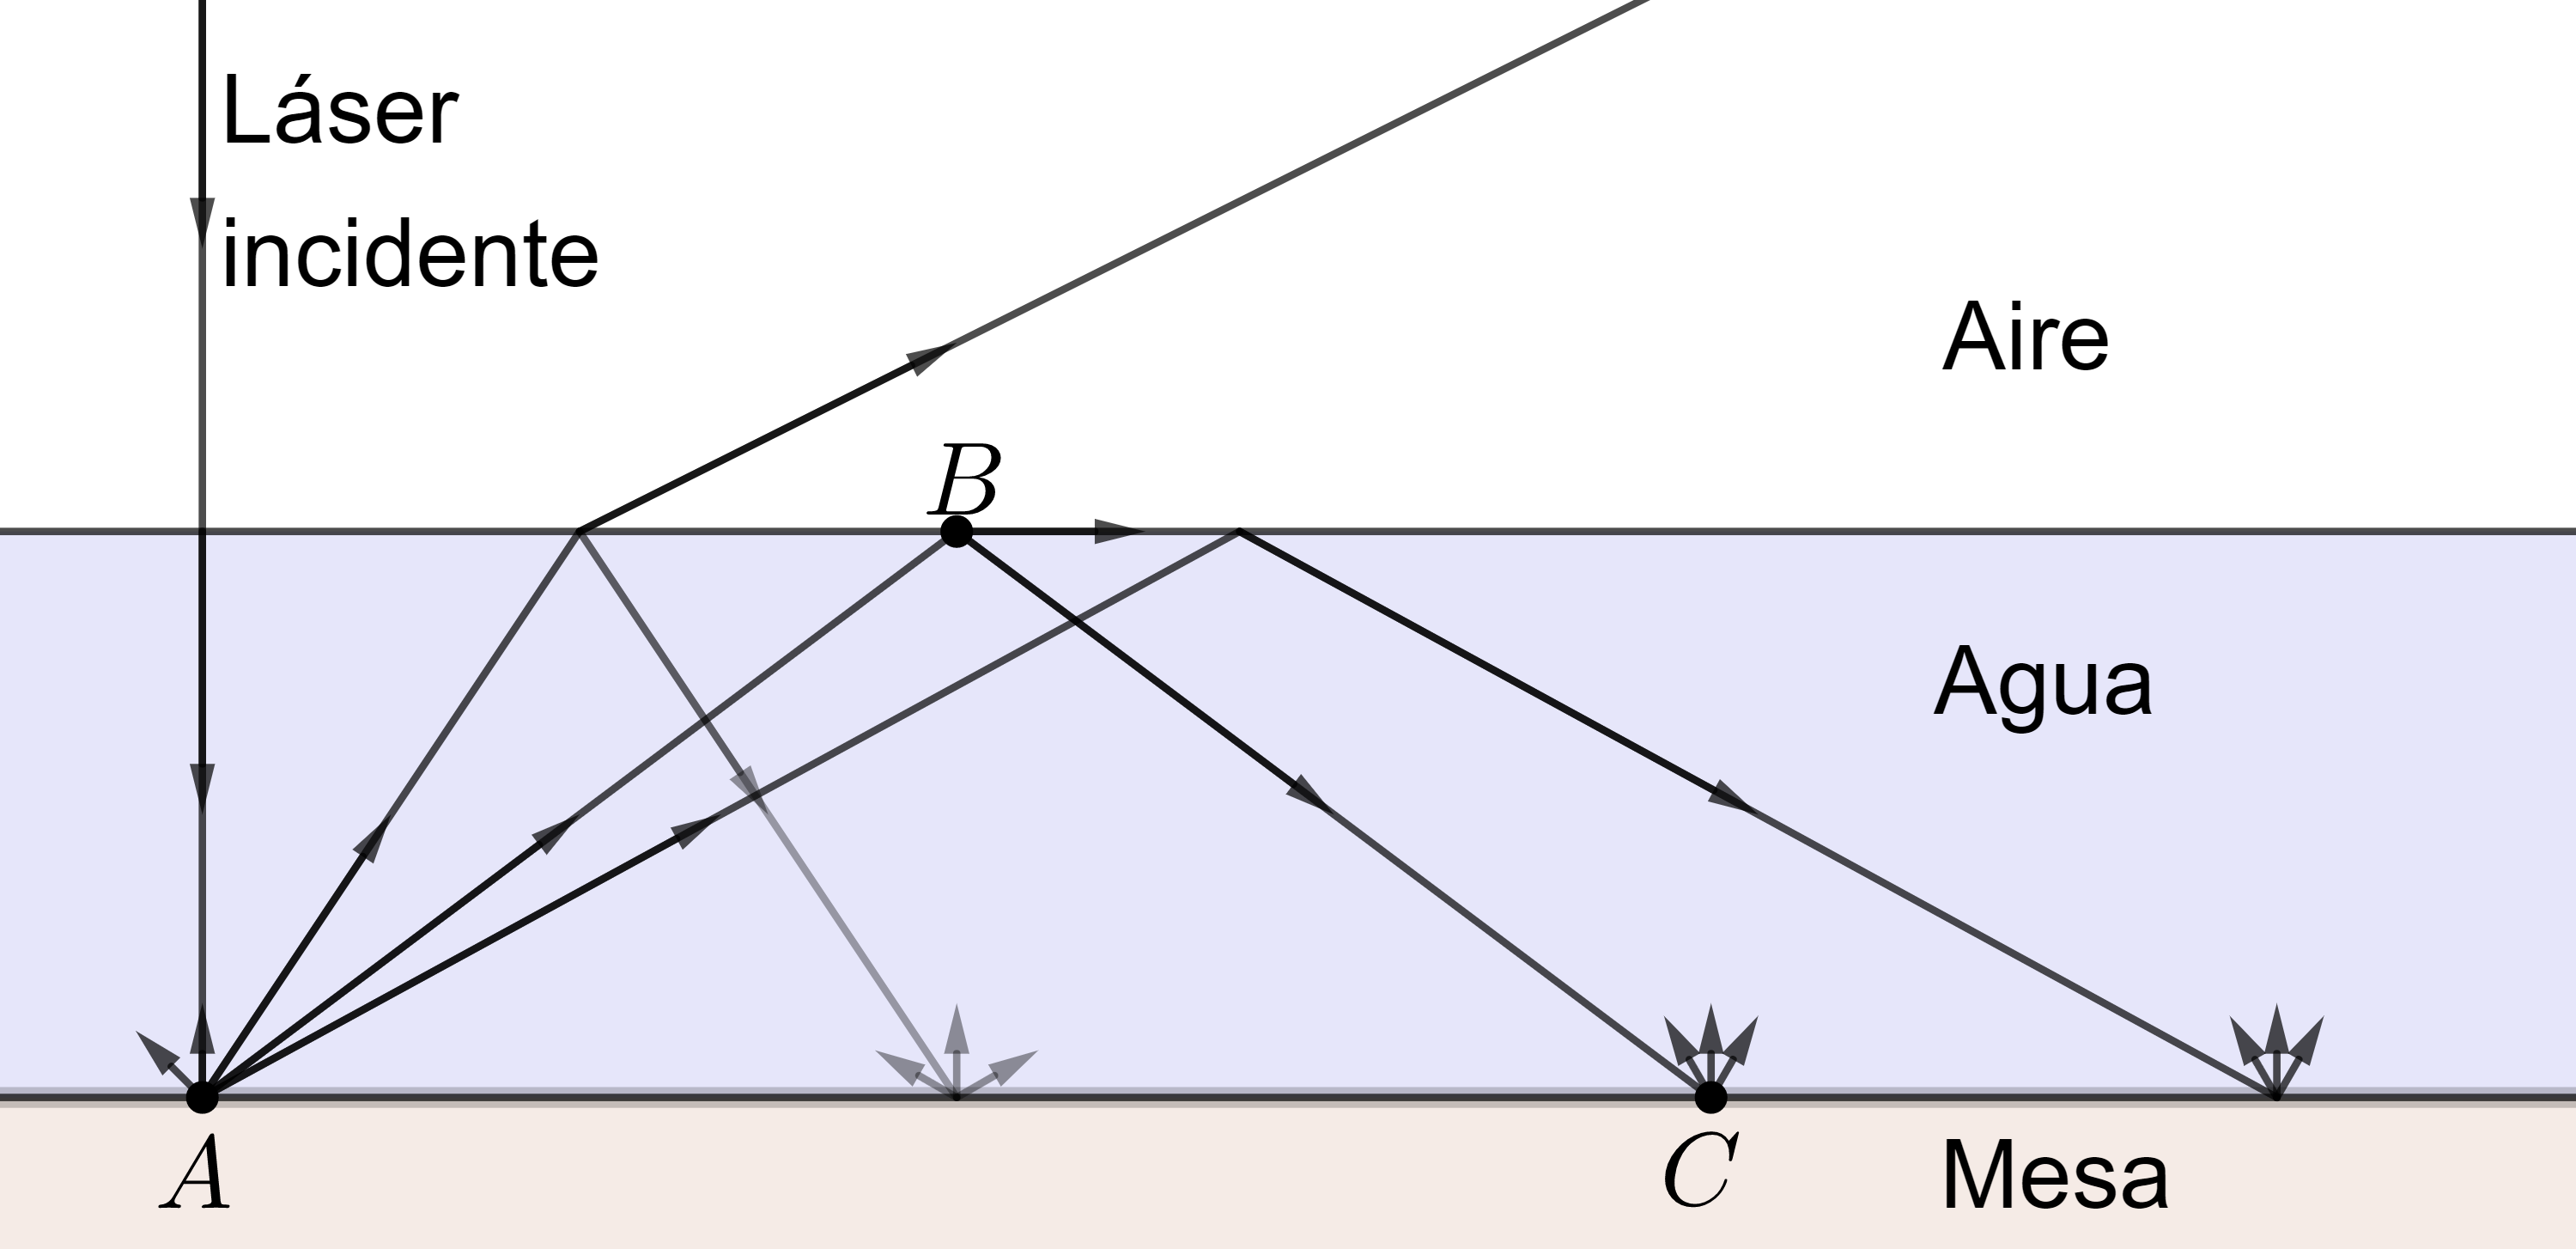
\includegraphics[width=10cm]{P2PffAgua.png}
		\caption{Esquema del efecto Pffund sobre una lámina de agua.}
		\label{P2PffAgua}
	\end{center}
\end{figure}

El rayo que llega a $B$ lo hace con un ángulo de incidencia igual al ángulo límite $\sen\varepsilon_l=\frac{1}{n}$ donde $n$ es el índice de refracción del agua (el del aire se considera 1). Si la distancia entre los puntos $A$ y $C$ es $r$, la distancia horizontal entre $A$ y $B$ es $\frac{r}{2}$. Si $d$ es el grosor de la lámina de agua, tenemos $\tan\varepsilon_l=\frac{r}{2d}$. Así pues el radio de la zona oscura es $r=2d\tan\varepsilon_l$ donde $\sen\varepsilon_l=\frac{1}{n}$.

\begin{equation}\label{P2PffRadioParvo}
	r=\frac{2d}{\sqrt{n^2-1}};\hspace{2mm}n=\sqrt{1+\frac{16d^2}{\phi^2}},\text{ donde }\phi=2r
\end{equation}

En resumen, en la gota se ve muy iluminado el punto $A$ sobre el que incide directamente el haz láser. Desde ese punto hasta el punto $C$ se ve una zona oscura y desde el punto $C$ hasta fuera de la gota se ve iluminado, aunque con menor intensidad, pues parte se ha perdido ya en la reflexión difusa del punto $A$.

La figura \ref{P2PffFotoAgua} es una fotografía que se hizo de este fenómeno. Se ve claramente un pequeño círculo brillante en el centro, luego una corona oscura y más allá otra corona brillante, lo cual concuerda con lo que se ha explicado de forma teórica.
\\

Ahora en lugar de una lámina de agua se pone una lámina de vidrio. Entre el vidrio y la mesa se forma una fina película de aire que cambia por completo lo que se observa. La figura \ref{P2PffVidrio} muestra un esquema de lo que les ocurre a los rayos. Sobre el punto $A$ se hace incidir el haz y de ahí se propaga en todas las direcciones. Los rayos que llegan a la cara superior de la lámina con un ángulo menor que el ángulo límite son en parte refractados y en parte reflejados. Su reflejo llega a la mesa y la ilumina. Sin embargo los rayos que llegan a la cara superior con un ángulo de incidencia igual ---o mayor--- al ángulo límite, son enteramente reflejados hacia abajo. Cuando llegan a la cara inferior de la lámina vuelven a llegar a una superficie de separación entre vidrio y aire. Por la ley de la refracción, al reflejarse el rayo en la cara superior sale con el mismo ángulo que el de incidencia, de modo que en la inferior el ángulo de incidencia es nuevamente el ángulo límite y el rayo se vuelve a reflejar totalmente. Así sucesivamente, dando lugar a una zona oscura.

Cuando se pone papel satinado en medio del camino del haz de luz, se dejan de ver los círculos y se pasa a ver una iluminación uniforme. Esto ocurre porque la luz atraviesa el papel, pero sale dispersa en todas las direcciones, mientras que sin el papel el haz de luz cae vertical.

\begin{figure}[!ht]
	\small \centering \sffamily
	\begin{center}
		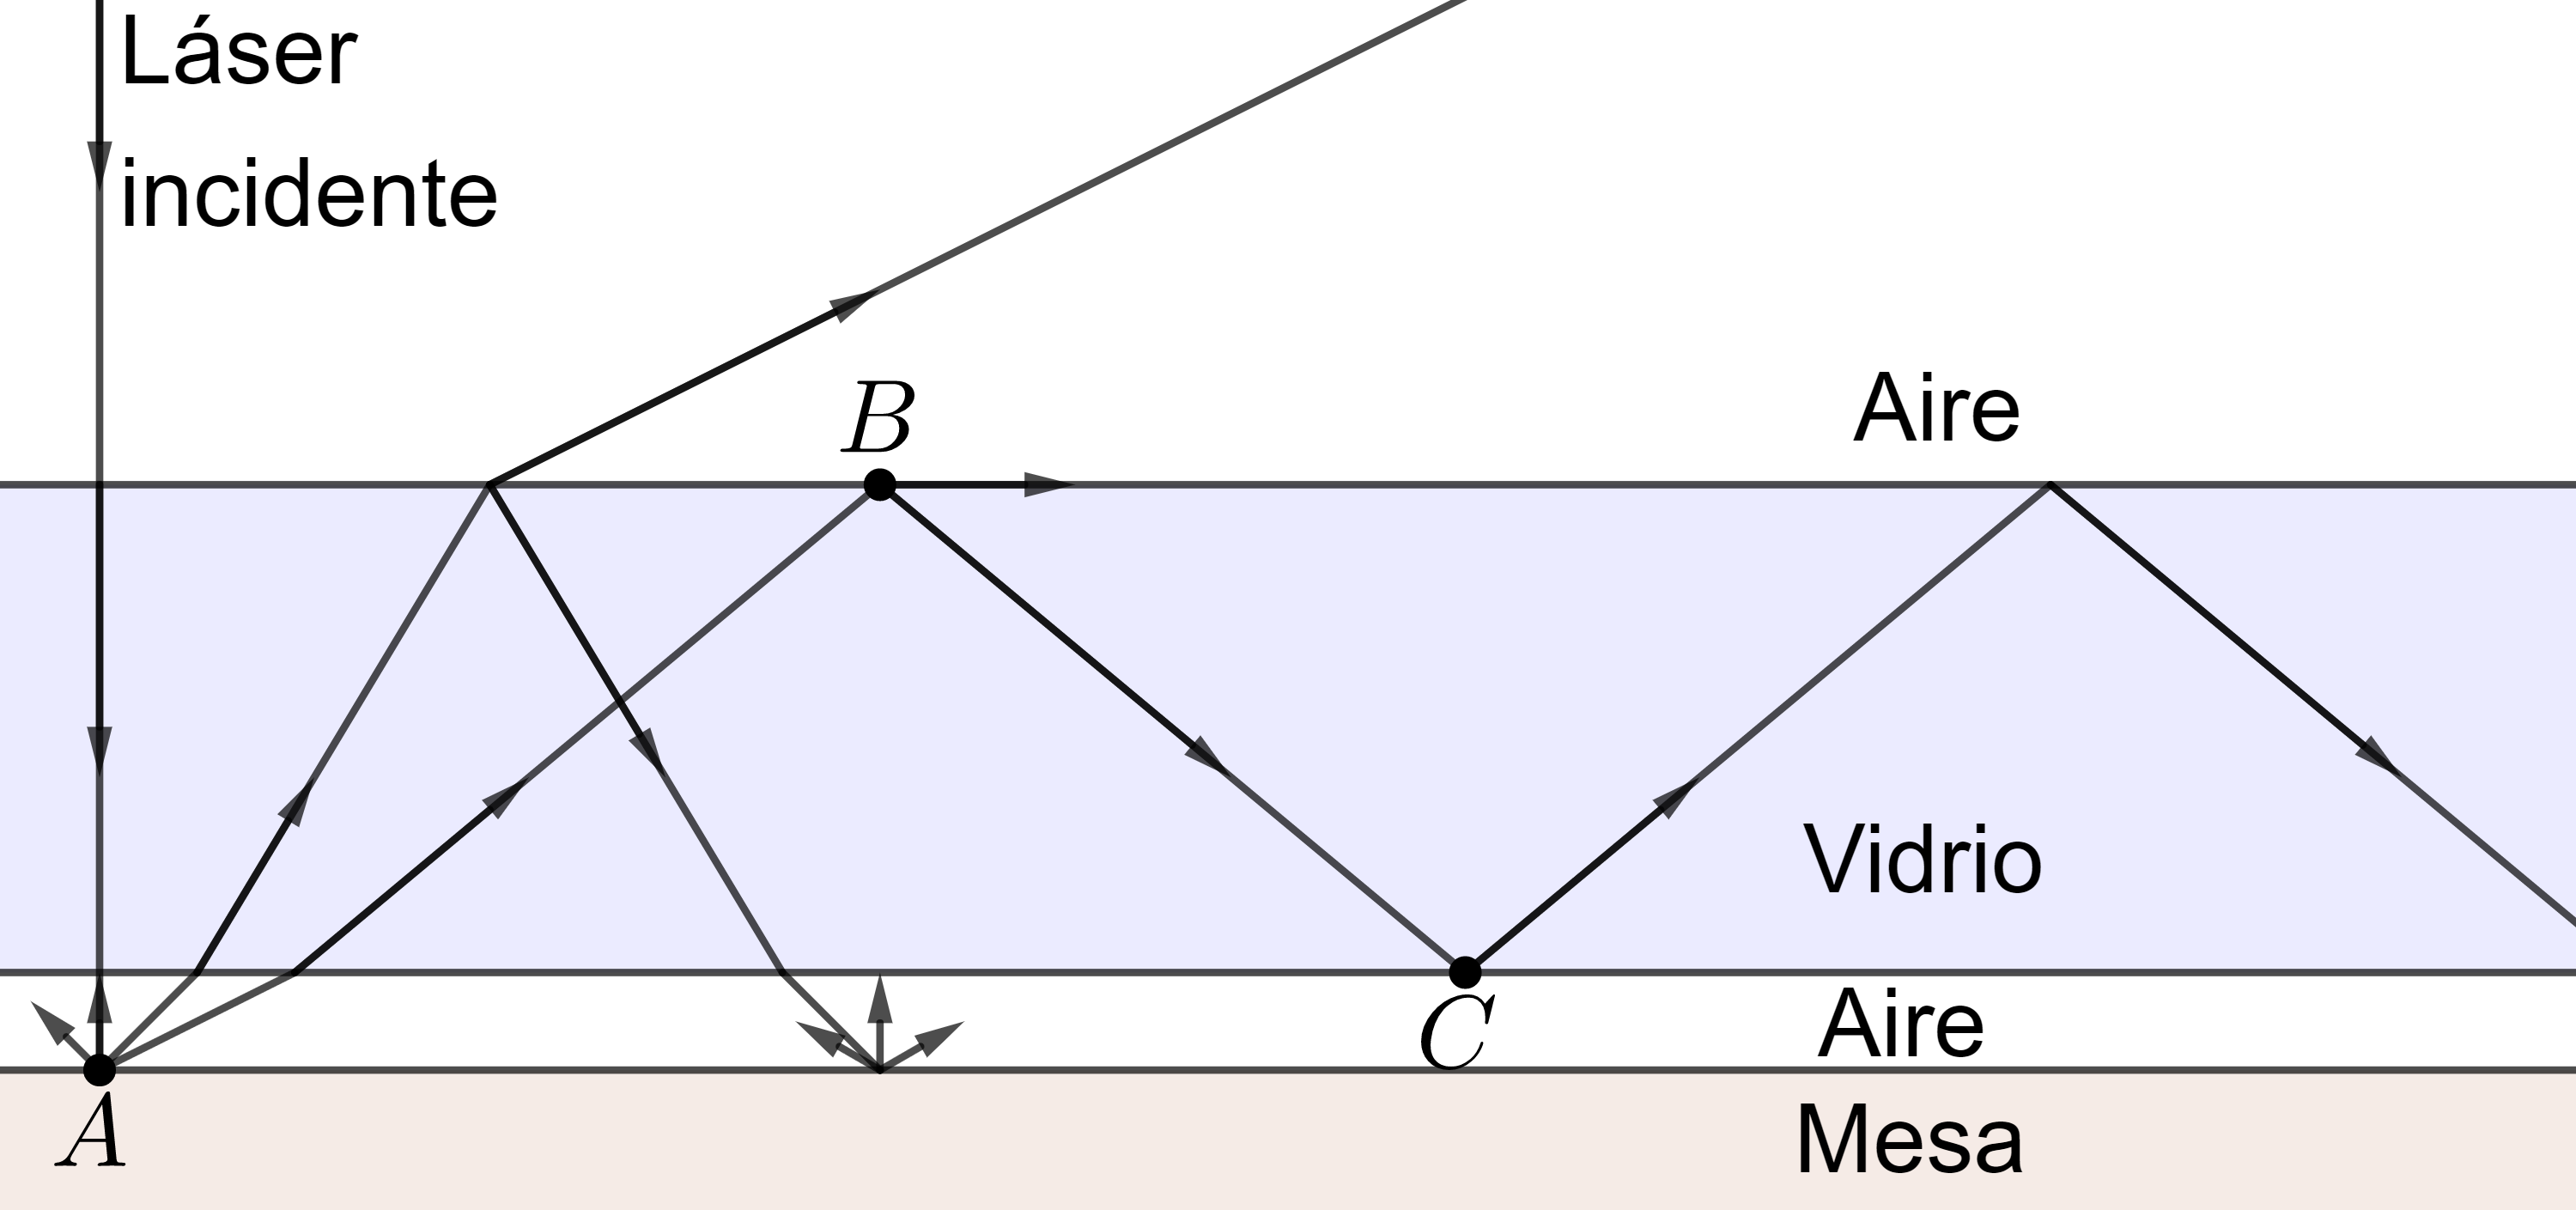
\includegraphics[width=10cm]{P2PffVidrio.png}
		\caption{Esquema del efecto Pffund sobre una lámina de vidrio.}
		\label{P2PffVidrio}
	\end{center}
\end{figure}

Por lo tanto se debería observar un punto central muy iluminado, una corona a su alrededor menos iluminada y más allá de la corona se vería oscuro. Como la capa de aire tiene un grosor despreciable, el radio de la zona iluminada viene dado por la misma ecuación (\ref{P2PffRadioParvo}) que en el caso anterior cambiando el índice de refracción del agua por el del vidrio ($n$) y el grosor de la capa de agua por el de la lámina de vidrio ($d$). Esto se ve claramente en la fotografía de la figura \ref{P2PffFotoVidrio} del anexo obtenida experimentalmente.

Se mide el diámetro de la zona iluminada, el cual es \data{1.80}{0.10}{cm} y el grosor de la placa de vidrio, que es \data{0.4670}{0.0010}{cm}. Con esto se calcula el índice de refracción de la lámina de vidrio utilizada con la ecuación (\ref{P2PffRadioParvo}) y su incertidumbre se calcula con la fórmula (\ref{P2incradioparvo}), dando un valor de $n_{\text{v}}=$\data{1.441}{0.042}{}.
\\

Si debajo de la lámina de vidrio se pone una fina capa de agua, a los rayos que salen con menor inclinación que el ángulo límite les sucede lo mismo: mayoritariamente se refractan y en una pequeña parte se reflejan; pero los que salen con más que el ángulo límite al llegar a la superficie vidrio-aire se reflejan totalmente y cuando llegan a la superficie vidrio-agua, como el índice de refracción del agua es mayor que el del aire, el rayo se refracta casi totalmente y acaba llegando a la mesa, sobre la cual se refleja de forma difusa.

El índice de refracción del vidrio es mayor que el del agua. Por lo tanto si el rayo de luz llega suficientemente oblicuo ---con un ángulo $\varepsilon_l'$--- del vidrio al agua se puede producir reflexión total. Estos rayos vuelven a la superficie vidrio-aire y se vuelven a reflejar totalmente, quedándose atrapados y originando una zona oscura.

\begin{figure}[!ht]
	\small \centering \sffamily
	\begin{center}
		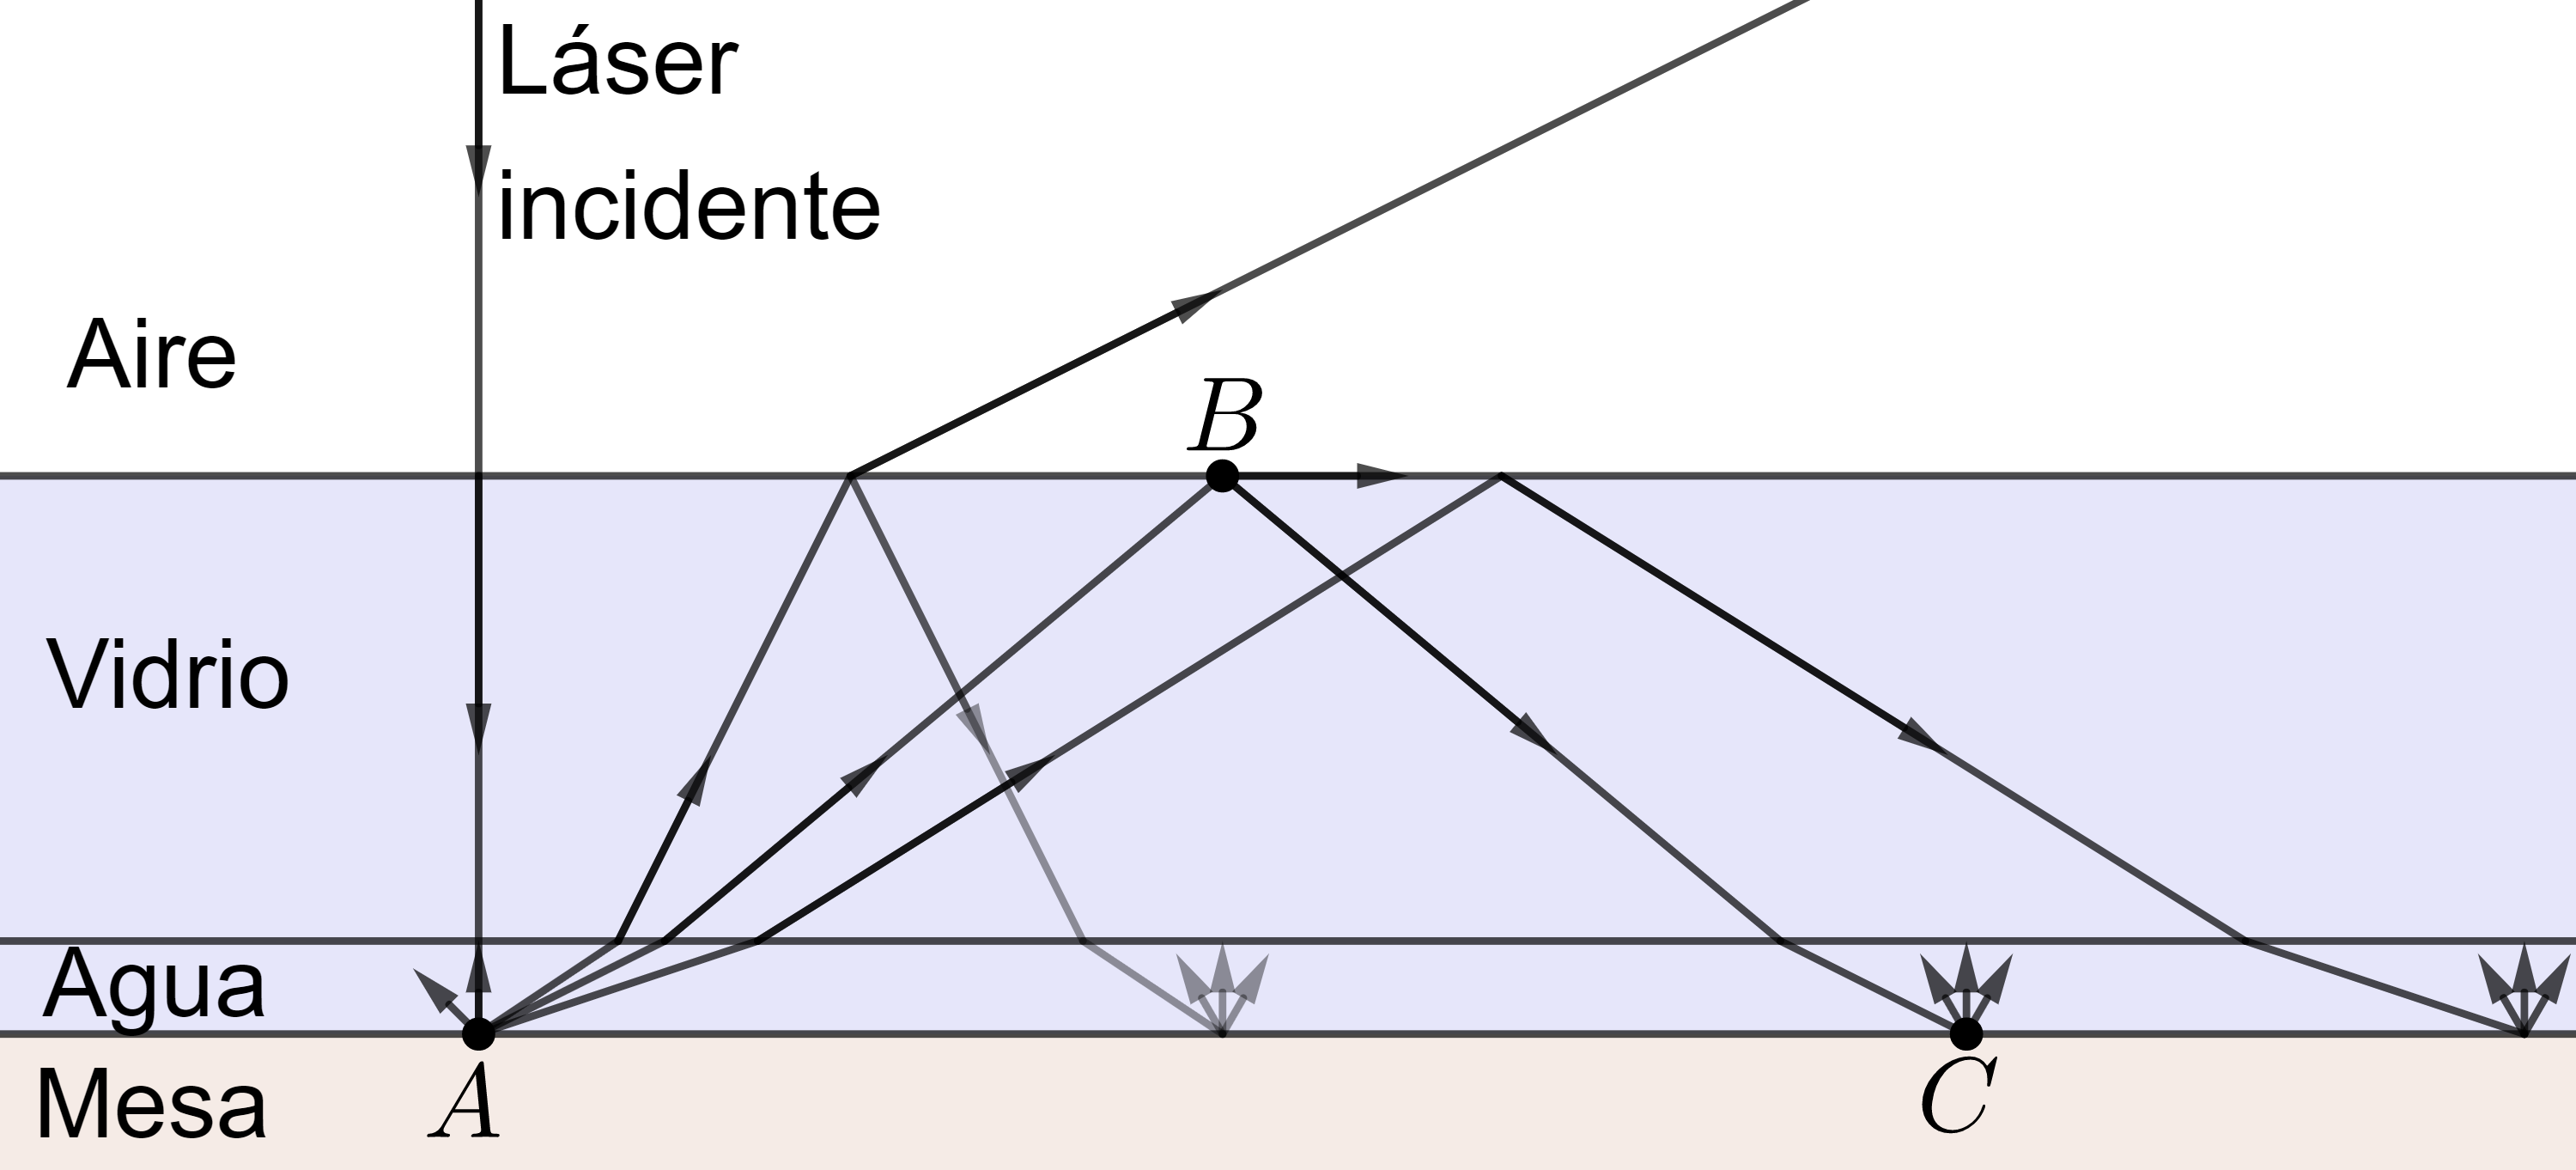
\includegraphics[width=10cm]{P2PffAgrio.png}
		\caption{Esquema del efecto Pffund sobre una lámina de vidrio que reposa sobre una capa de agua.}
		\label{P2PffAgrio}
	\end{center}
\end{figure}

En la fotografía de la figura \ref{P2PffFotoAgrio} se ve un punto central muy iluminado, una corona oscura a su alrededor, fuera de ella se ve una corona más grande iluminada y más allá de ella se queda oscuro. El radio de la corona oscura $r_1$ se calcula con la fórmula (\ref{P2PffRadioParvo}) siendo $n$ y $d$ los parámetros de la lámina de vidrio.

La corona iluminada se acaba donde el rayo de luz tiene un ángulo incidente $\varepsilon_l'$. $\sen\varepsilon_l'=\frac{n_\text{a}}{n_\text{v}}$. Con esto se puede calcular el radio de la corona iluminada.

\begin{equation}\label{P2PffRadioMagno}
	r=\frac{2d}{\sqrt{\left(\frac{n_\text{v}}{n_\text{a}}\right)^2-1}};\hspace{2mm}n_\text{a}=\frac{n_\text{v}}{\sqrt{1+\frac{16d^2}{\phi^2}}}
\end{equation}

Si hay una burbuja, los rayos que llegan a ella son desviados y la zona de donde salen estos se queda oscura. En lugar de ver el punto de donde salen los rayos, vemos la imagen de donde parecen venir los rayos, la cual vemos en otro lugar. Se puede ver esto en el esquema de la figura \ref{P2PffBurbuja}. El punto $A$ se ve perfectamente, pero el punto $O$ se ve oscuro porque en su lugar su imagen $O'$, que se debería ver oscura se ve iluminada.

\begin{figure}[!ht]
	\small \centering \sffamily
	\begin{center}
		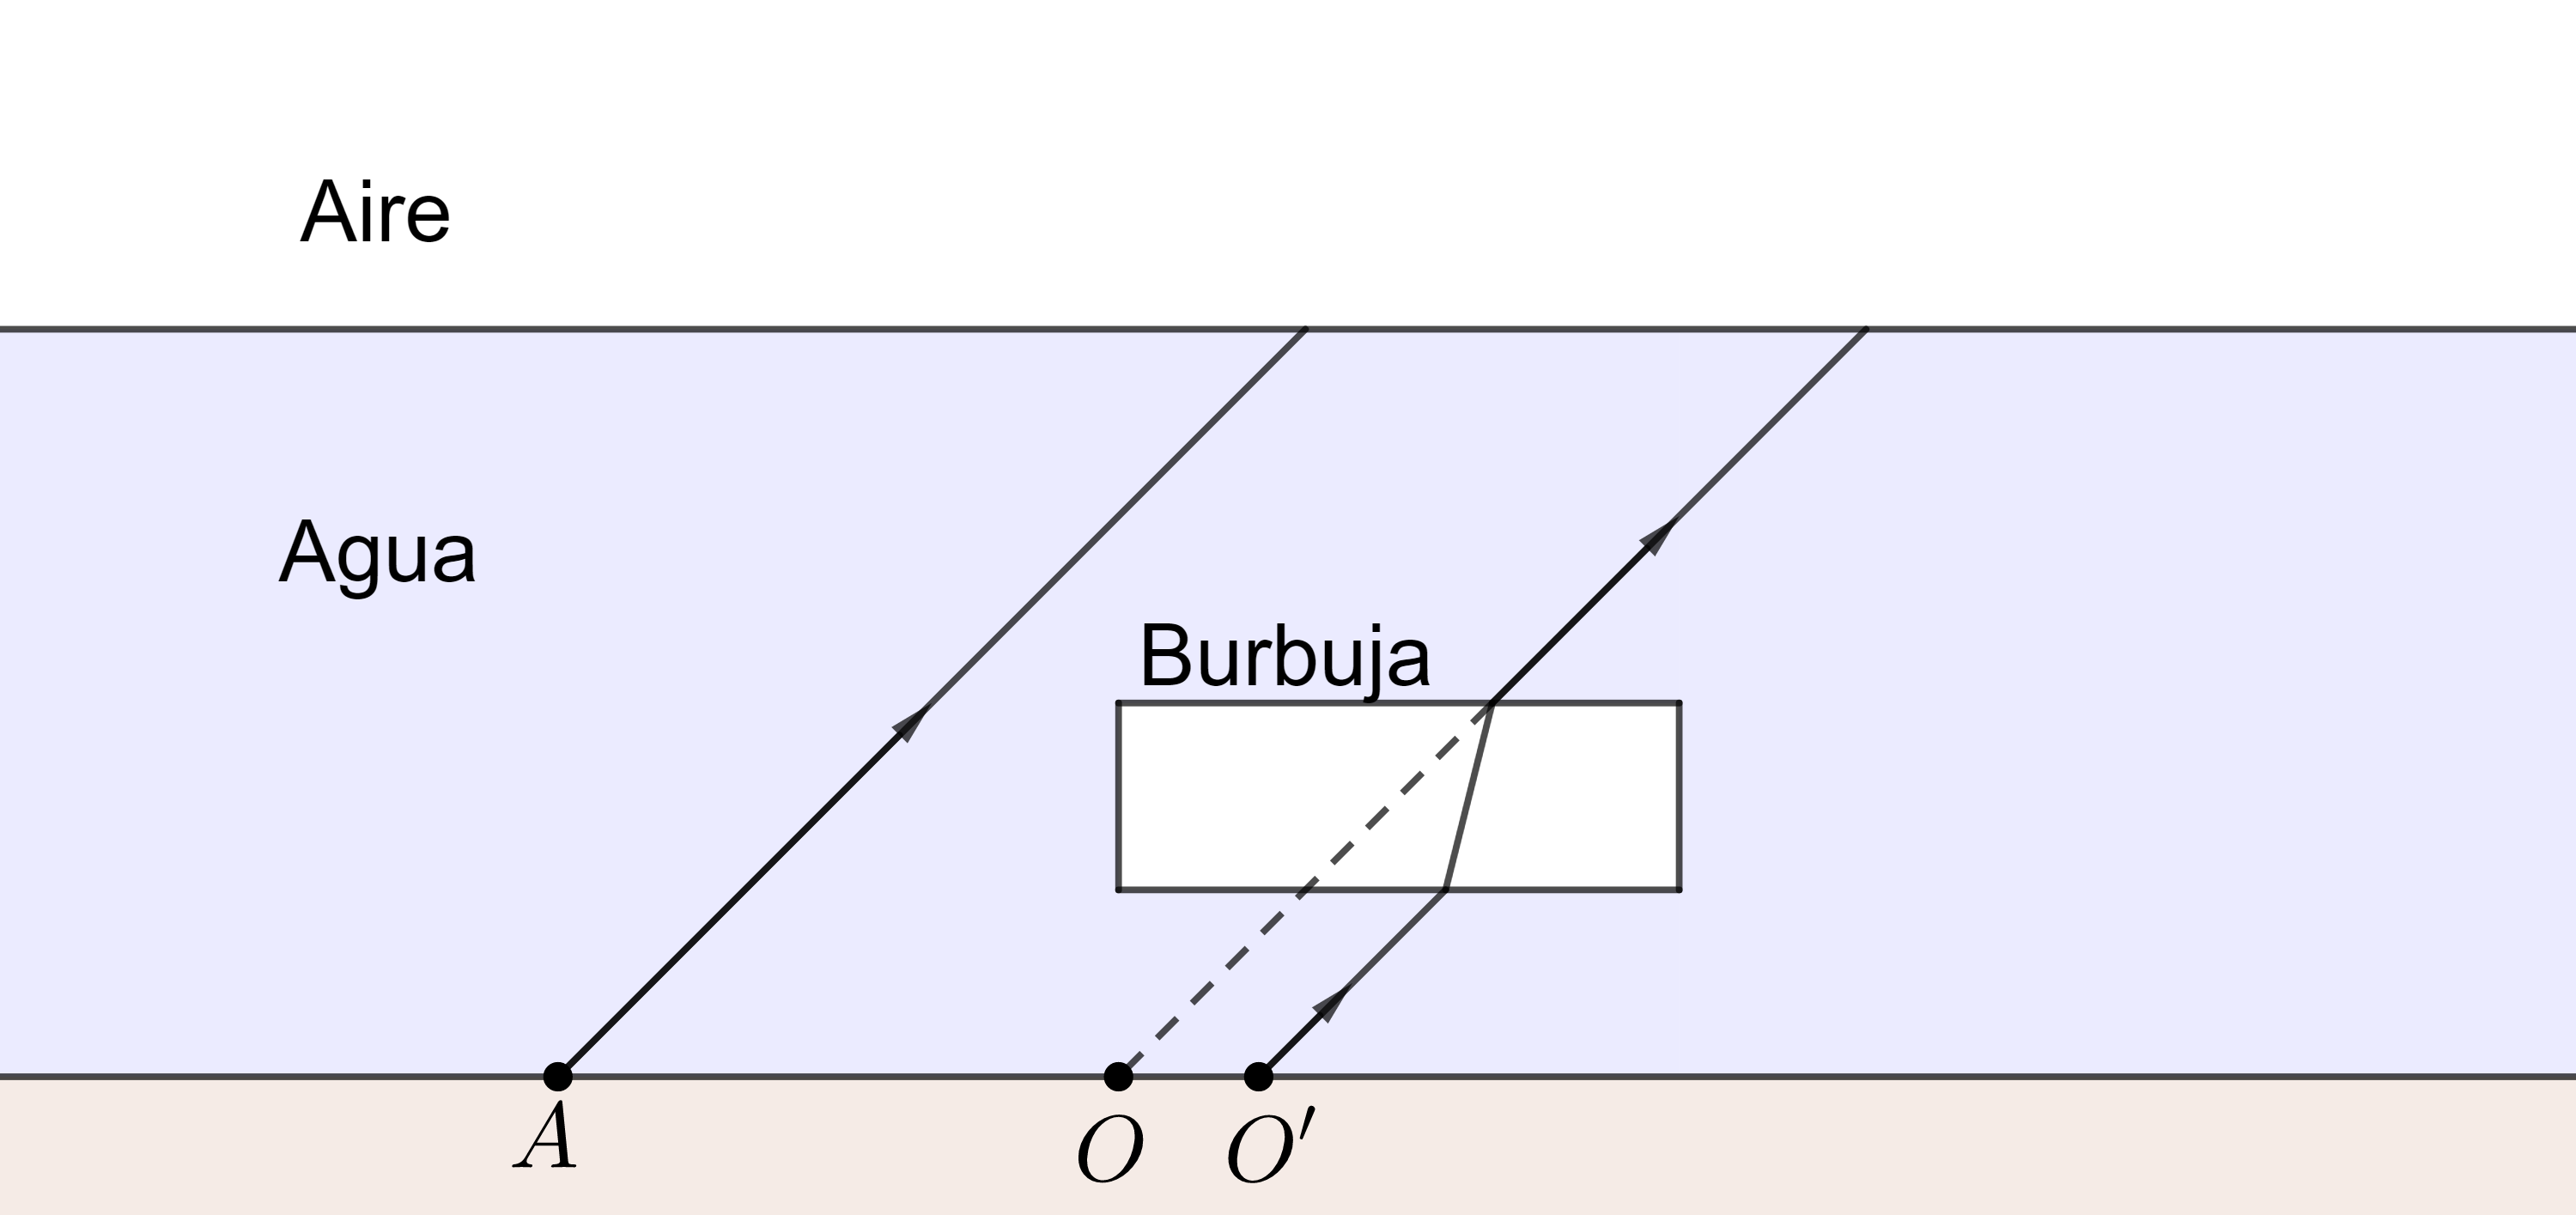
\includegraphics[width=10cm]{P2PffBurbuja.png}
		\caption{Esquema del efecto de una burbuja sobre los rayos que llegan al ojo.}
		\label{P2PffBurbuja}
	\end{center}
\end{figure}

Una fotografía tomada de este caso y que confirma lo que se ha explicado se encuentra en la figura \ref{P2PffFotoVidrio}. Se ve el punto central brillante, una corona oscura y otra iluminada. Además se ve que hay una pequeña burbuja, pues los rayos que vienen de la mancha negra son desviados y parecen venir de la mancha iluminada que hay un poco más arriba en la fotografía.

En este caso se mide el diámetro de la corona iluminada, el cual es \data{3.70}{0.10}{cm}. Se recuerda que el grosor de la placa de vidrio es \data{0.4670}{0.0010}{cm} y que se ha calculado ya $n_{\text{v}}=$\data{1.441}{0.042}{}. Así con la fórmula (\ref{P2PffRadioMagno}) se calcula el índice de refracción del agua y con la fórmula (\ref{P2incradiomagno}), obteniéndose un índice $n_{\text{a}}=$\data{1.287}{0.038}{}.
\\

Cuando se vierte agua sobre la lámina de vidrio el proceso que ocurre es el mismo, y se visualiza en la figura \ref{P2PffAgria}, solo que el medio limítrofe con el aire es el agua, por lo que en la fórmula (\ref{P2PffRadioParvo}) del radio de la corona oscura se debe poner el índice de refracción del agua en lugar del del vidrio. Como los índices del agua y del vidrio son parecidos no se aprecia una gran diferencia en el radio. El radio de la corona iluminada, por su parte, permanece igual.

\begin{figure}[!ht]
	\small \centering \sffamily
	\begin{center}
		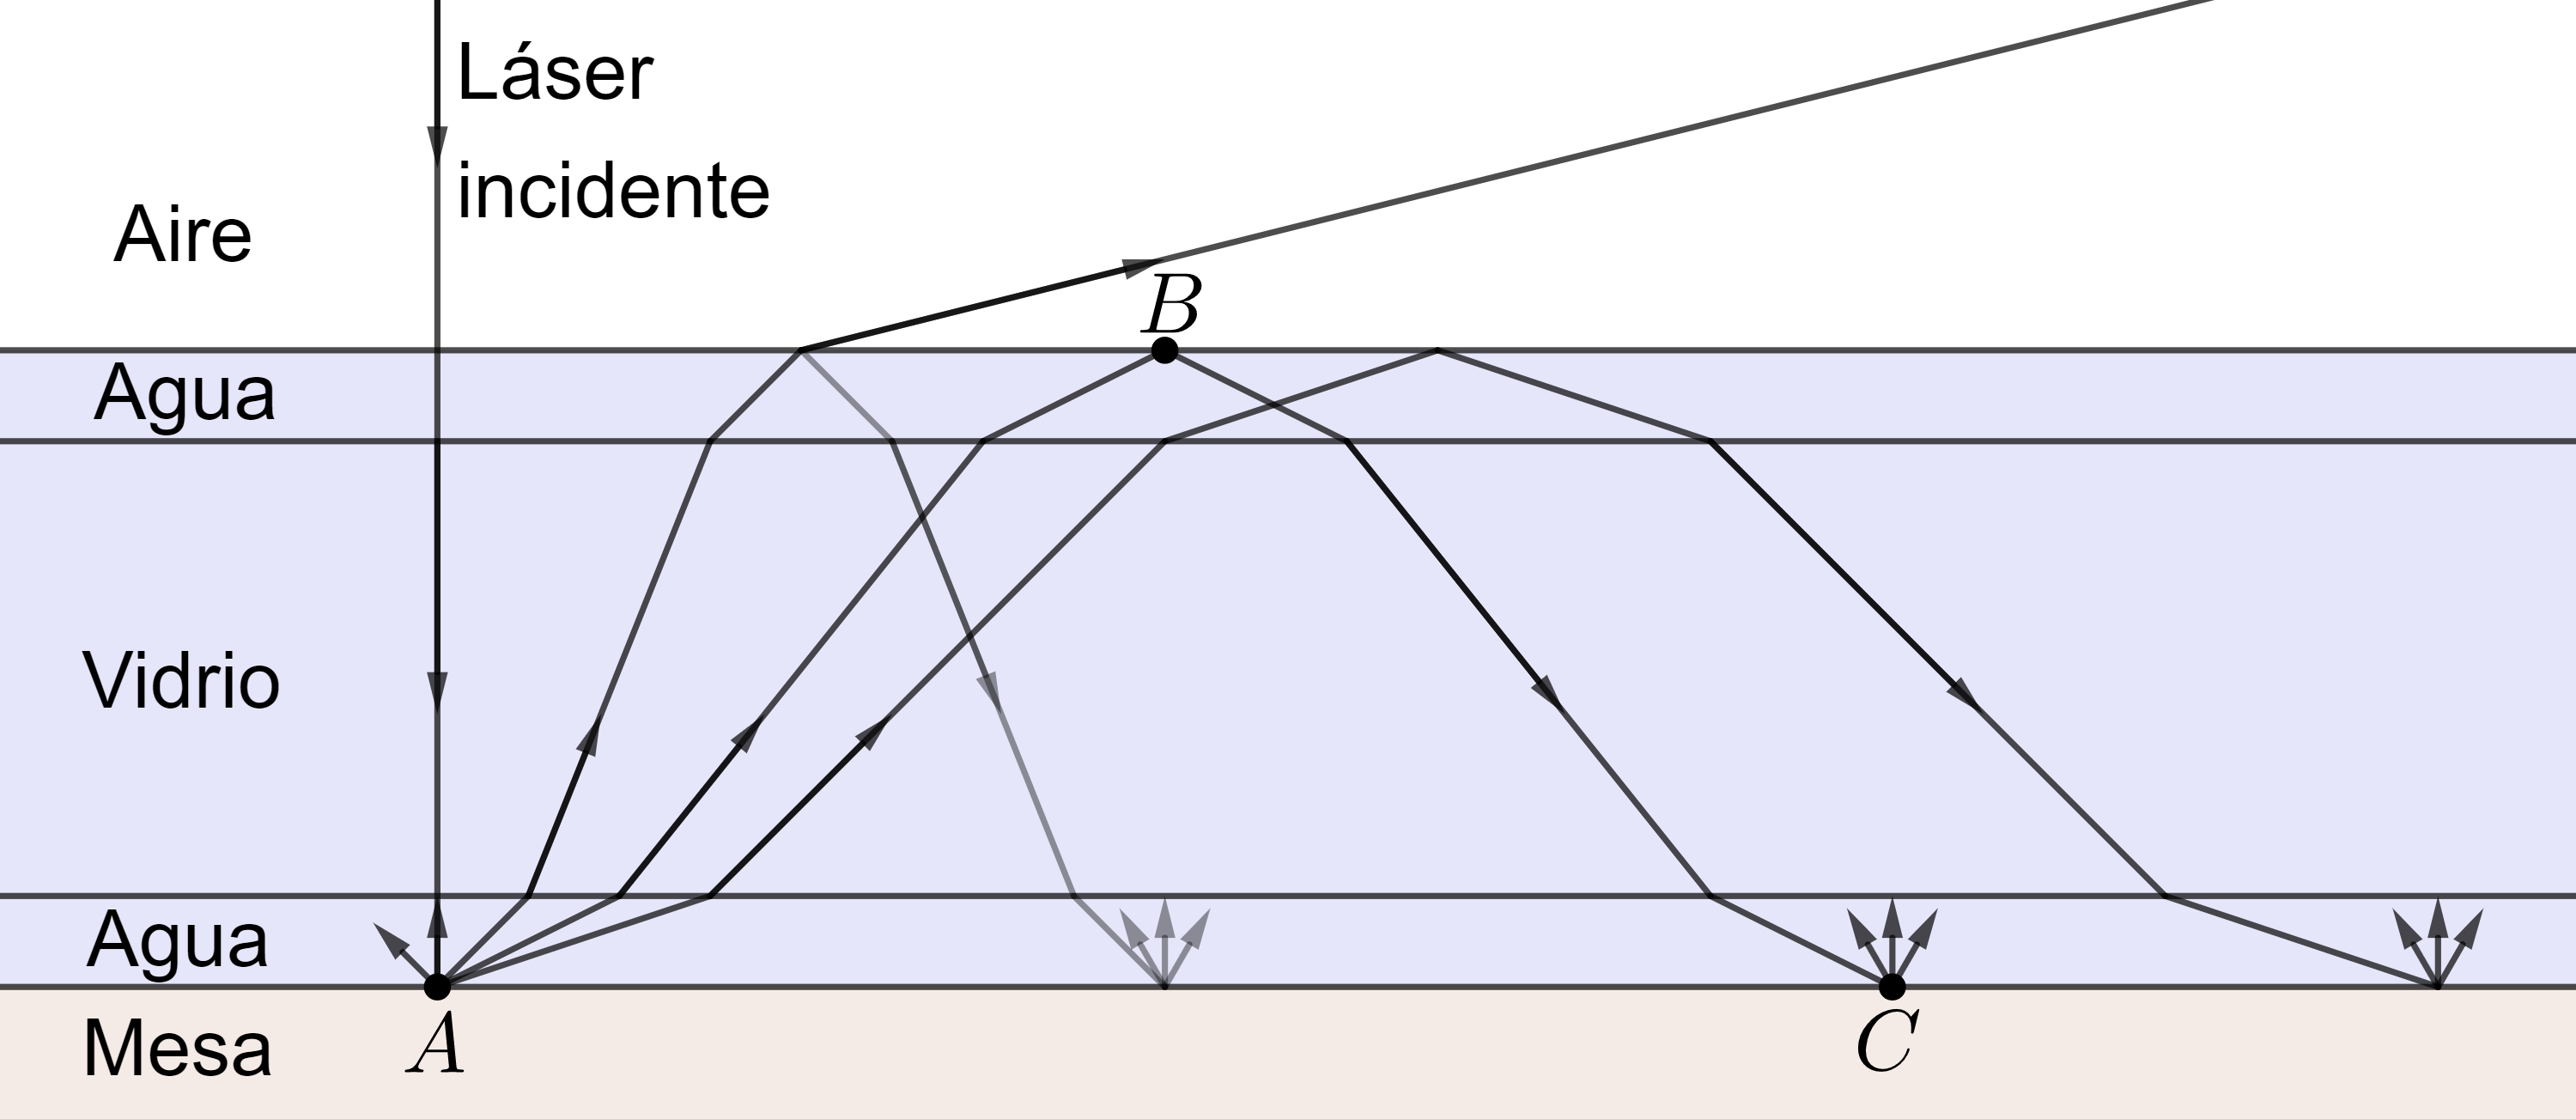
\includegraphics[width=10cm]{P2PffAgria.png}
		\caption{Esquema del efecto Pffund sobre una lámina de vidrio que se encuentra entre dos capas de agua.}
		\label{P2PffAgria}
	\end{center}
\end{figure}

En cada caso han tenido lugar los siguientes fenómenos ópticos.
\begin{enumerate}
	\item Luz sobre la mesa. Reflexión difusa.
	\item Espejo por el lado de aluminio. Reflexión especular.
	\item Papel satinado. Reflexión difusa y refracción.
	\item Plástico. Reflexión difusa.
	\item Espejo por el lado de vidrio. Refracción y reflexión especular.
	\item Efecto Pffund.
		\begin{itemize}
			\item Reflexión difusa sobre la mesa
			\item Reflexión especular en las superficies agua-aire, vidrio-aire, vidrio-agua.
			\item Reflexión total del agua al aire, del vidrio al aire y del vidrio al agua.
			\item Refracción en las superficies agua-aire, vidrio-aire, vidrio-agua.
		\end{itemize}
\end{enumerate}

\section{Conclusiones}
En los fenómenos de refracción y reflexión de la luz, esta se puede entender como una serie de rayos que se propagan en línea recta, pues explican todos los resultados observados en esta práctica.

Cuando un objeto emite rayos que se refractan en un dioptrio plano, se forma una imagen que en el caso paraxial será nítida. Esta imagen es la que se ve con el ojo. Gracias a esto se ha podido calcular el índice de refracción de una lámina de vidrio. Se ha comprobado asimismo la dependencia del mismo con la longitud de onda de la luz empleada, lo cual genera una dispersión cromática, la cual en algunos casos no es despreciable y puede llegar a generar aberraciones cromáticas que impidan formar una imagen con claridad.

Se ha visto también que no se ve el rayo de luz, sino el punto de donde proviene. Esto quiere decir que si un rayo sale de una fuente en una dirección y se refleja especularmente, pero no termina en el ojo, no se verá nada.

Además no todas las superficies son iguales: en algunas los rayos de luz se refractan, en otras se reflejan especular o difusamente, a veces una parte es refractada y otra reflejada... Esto da lugar al efecto Pffund, el cual utiliza conceptos de reflexión total y materiales de distintos índices de refracción para explicar las formas que se ven al iluminarlos. El efecto se ha podido comprobar satisfatoriamente en el laboratorio, permitiendo calcular los índices de refracción del vidrio y del agua.

Se puede concluir que la óptica geométrica es fundamental a la hora de explicar la propagación de la luz. Es capaz de explicar una gran cantidad de fenómenos que se producen cuando la luz llega a superficies de separación entre dos medios.

\begin{thebibliography}{1}
\bibitem{P2bibguion} \textsc{Grupo de óptica, departamento de física.} \textit{Guión de la práctica 2}. Universidad Autónoma de Barcelona, 2018.
\end{thebibliography}
\newpage

\appendix
\section{Cálculo de incertidumbres}
La incertidumbre $u_{x-y}$ de la diferencia entre dos medidas de igual incertidumbre $u_x=u_y=u_0$ es
\begin{equation}\label{P2incdif}
u_{x-y}^2=\sqrt{\left(\frac{\partial(x-y)}{\partial x}\right)^2u_x^2+\left(\frac{\partial(x-y)}{\partial y}\right)^2u_y^2}=\sqrt{u_x^2+u_y^2}=\sqrt{2u_0^2}=\sqrt{2}u_0.
\end{equation}

Cuando se tienen diversas medidas de una misma magnitud, la incertidumbre estadística $u_{\text{est}}$ de la media es 
\begin{equation}\label{P2incest}
u_{\text{est}}^2=\frac{1}{n(n-1)}\sum_{i=1}^n(x_i-\bar{x})^2,\hspace{3mm}\text{donde }\bar{x}=\frac{1}{n}\sum_{i=1}^nx_i
\end{equation}
Para obtener su incertidumbre total $u_{\text{tot}}$ hay que sumar la incertidumbre instrumental $u_{\text{exp}}$ de las medidas.
\begin{equation}\label{P2incmedia}
u_{\text{tot}}=\sqrt{u_{\text{est}}^2+u_{\text{inc}}^2}
\end{equation}

Recuérdese la fórmula de propagación de incertidumbres de una función escalar $y=f(x_1,\ldots,x_n)$.
\begin{equation}\label{P2incprop}
u_y^2=\sum_{i=1}^n\left(\frac{\partial f}{\partial x_i}\right)^2u_i^2
\end{equation}

Para calcular la incertidumbre de $n$ de la fórmula \ref{P2PffRadioParvo} se utiliza la propagación de incertidumbres.
\begin{equation}\label{P2incradioparvo}
u_n=\frac{16d}{\Phi^2\sqrt{1+\frac{16d^2}{\Phi^2}}}\sqrt{u_d^2+\frac{d^2}{\Phi^2}u_\Phi^2}
\end{equation}

Para calcular la incertidumbre de $n$ de la fórmula \ref{P2PffRadioMagno} se utiliza la propagación de incertidumbres.
\begin{equation}\label{P2incradiomagno}
\frac{1}{\sqrt{1+\frac{16d^2}{\Phi^2}}}\sqrt{u_{n_\text{v}}^2+\frac{n_\text{v}}{\left(1+\frac{16d^2}{\Phi^2}\right)^2}\cdot\frac{256d^2}{\Phi^4}\left(u_d^2+\frac{d^2}{\Phi^2}u_\Phi^2\right)}
\end{equation}

\newpage
\section{Fotografías}

\begin{figure}[!ht]
	\small \centering \sffamily
	\begin{center}
		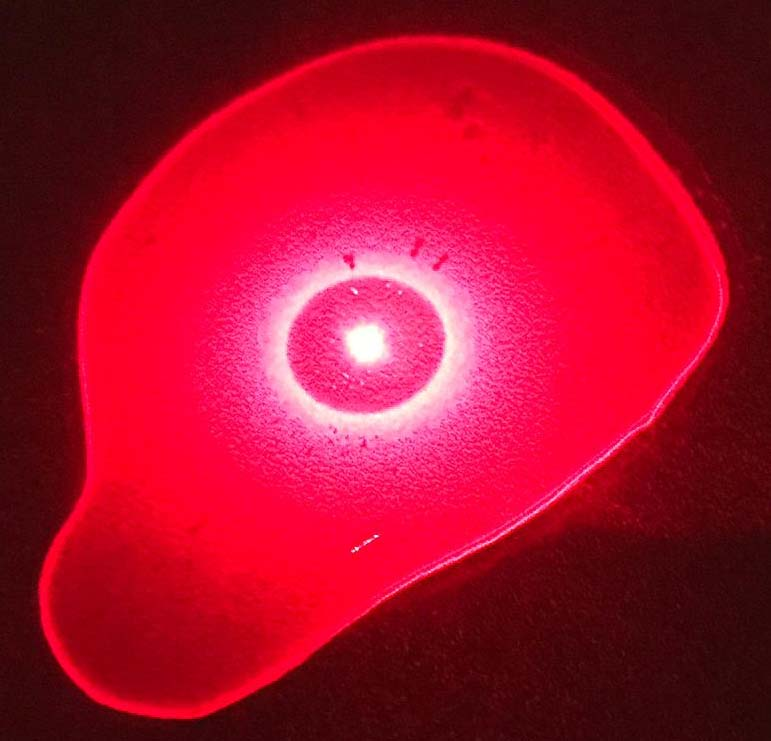
\includegraphics[scale = 0.15]{P2PffAgua.jpeg}
		\caption{Fotografía de una superficie de agua sobre la mesa iluminada con un rayo láser ilustrando el efecto Pffund.}
		\label{P2PffFotoAgua}
	\end{center}
\end{figure}

\begin{figure}[!ht]
	\small \centering \sffamily
	\begin{center}
		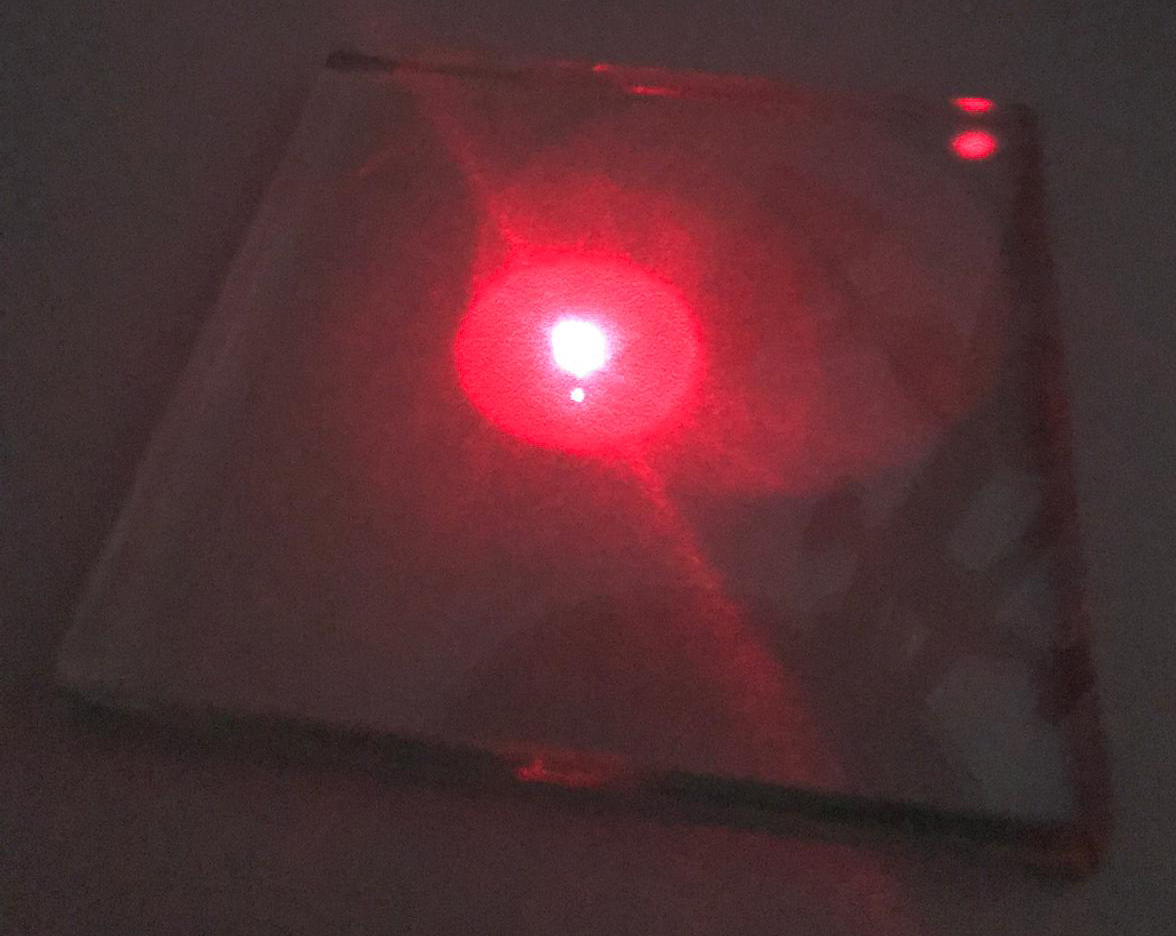
\includegraphics[scale = 0.15]{P2PffVidrio.jpeg}
		\caption{Fotografía de una lámina de vidrio sobre la mesa iluminada con un rayo láser ilustrando el efecto Pffund.}
		\label{P2PffFotoVidrio}
	\end{center}
\end{figure}

\begin{figure}[!ht]
	\small \centering \sffamily
	\begin{center}
		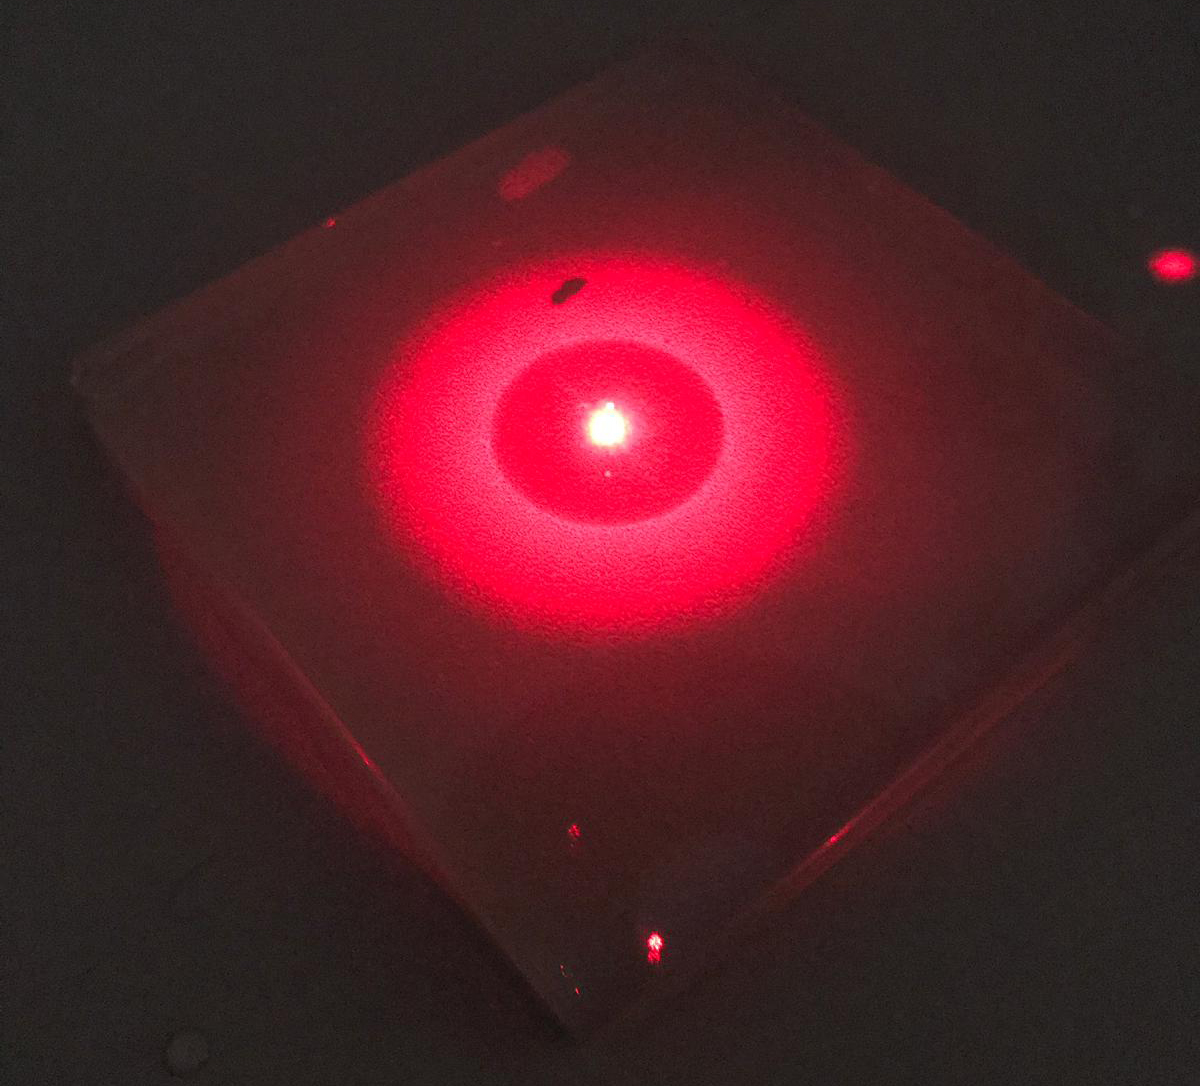
\includegraphics[scale = 0.15]{P2PffAgrio.jpeg}
		\caption{Fotografía de una lámina de vidrio sobre una capa de agua sobre la mesa iluminada con un rayo láser ilustrando el efecto Pffund.}
		\label{P2PffFotoAgrio}
	\end{center}
\end{figure}

\end{document}
